% ===================================================================
% CONFIGURACIÓN DEL DOCUMENTO
% ===================================================================
\documentclass[conference]{IEEEtran}
\IEEEoverridecommandlockouts % Permite usar \thanks en el bloque de autores

% Carga el preámbulo con paquetes y configuraciones comunes
\input{preamble.tex}

% Definición del comando BibTeX para la bibliografía (estándar de IEEE)
\def\BibTeX{{\rm B\kern-.05em{\sc i\kern-.025em b}\kern-.08em
  T\kern-.1667em\lower.7ex\hbox{E}\kern-.125emX}}

% ===================================================================
% INICIO DEL DOCUMENTO
% ===================================================================
\begin{document}
  % Configuración de los colores para los hipervínculos del PDF
  % Para revisiones a doble ciego, se recomienda usar 'black' en todos los campos.
  \hypersetup{citecolor=black, linkcolor=black!80, urlcolor=gray, breaklinks=true}

  % ===================================================================
  % TÍTULO Y AUTORES
  % ===================================================================
  % Edita el título del artículo aquí.
  \title{Bitácoras Sistemas Embebidos Primer Corte\\\vspace{2pt}}

  % Edita la información de los autores.
  % Duplica el bloque \IEEEauthorblock para añadir más autores y afiliaciones.
  % En envíos anónimos (doble ciego), elimina esta sección o anonimiza los datos.
  \author{
  \IEEEauthorblockN{Julian Díaz Cortina}
  \IEEEauthorblockA{\textit{Ingeniería Mecatrónica}\\
    \textit{Universidad Santo Tomás}\\
    Bucaramanga, Colombia\\
    juliandavid.diaz@ustabuca.edu.co}
  \and
  \IEEEauthorblockN{Fabian Ruiz Mateus}
  \IEEEauthorblockA{\textit{Ingeniería Mecatrónica}\\
    \textit{Universidad Santo Tomás}\\
    Bucaramanga, Colombia\\
    fabianaugusto.ruiz@ustabuca.edu.co}
  }

  % Descomenta la siguiente línea para añadir notas de financiación o agradecimientos en el pie de página del título.
  % \thanks{Este trabajo fue financiado por la Institución XYZ bajo el proyecto ABC.}

\maketitle

% Ajuste de estilo para mantener la tipografía original de IEEE.
\renewcommand\sffamily{}

% ===================================================================
% RESUMEN Y PALABRAS CLAVE
% ===================================================================
% El contenido del resumen y las palabras clave se encuentra en 'abstract.tex'.
\input{section/abstract}

% ===================================================================
% CUERPO DEL ARTÍCULO
% ===================================================================
% Se recomienda organizar cada sección en un archivo .tex separado para mayor claridad.
% Usa \label{sec:nombre} para crear etiquetas y \ref{sec:nombre} para referenciarlas.

\section{Introducción}\label{sec:introduccion}
  \input{section/introduction}

% Descomenta la siguiente sección para incluir una revisión del estado del arte.
% Asegúrate de crear y editar el archivo 'literature.tex'.
 %\section{Revisión de literatura}\label{sec:literatura}
  \input{section/literature}

\section{Marco referencial}\label{sec:experimental}
    % Esta sección describe equipo y procedimiento de manera simple.
% Reemplaza con tu propio contenido cuando enseñes o evalúes.

\subsection{Actividad 1} % Sub-sección (nivel bajo \section) para detallar hardware

\subsubsection{Caso de estudio}

Se desea diseñar un sistema basado en microcontrolador que:
\begin{itemize}
    \item Lea un sensor cada 10 ms.
    \item Controle un motor según la lectura.
    \item Envíe datos por comunicación serial cada 100 ms.
    \item Atienda un botón de emergencia que debe detener todo inmediatamente.
    \item Muestre información en una pantalla.
\end{itemize}
\vspace{0.3cm}
\begin{itemize}
    \item\textbf{ ¿Cómo implementar esto usando solo un while?:}
    La respuesta de esta pregunta genera como resultado el diagrama de flujo que se encuentra en la figura \ref{Diagrama de flujo}.
     
    \vspace{0.3cm}
    \item \textbf{¿Qué problemas podrían aparecer?:} Al ser un while con dependencia doble, interna y distinta del tiempo; se puede estar presentando retrasos de lectura, pues la lectura lineal debe esperar a, por ejemplo, enviar el paquete de datos por el puerto serial para continuar con el proceso. Esto mismo trae problemas de latencia y de estabilidad, pues en el caso que se desee agregar mas tareas, el control del tiempo se verá aún mas afectado.
    \vspace{0.3cm}
    \item \textbf{¿Qué tarea sería más crítica?:} En este caso desarrollado, se entiende que la tarea más critica seria toda la que conlleve al botón de emergencia, pues estamos hablando de factores de seguridad humana y estos deben ser considerados de manera prioritaria.
    \vspace{0.3cm}
    \item \textbf{¿Cómo garantizarías tiempos de respuesta?:} En una primera parte, se deberían independizar dos elementos claves: La parada de emergencia y el timer, pues estos deben ser independientes de una revisión ocasional dentro del while. Una manera de hacerlo es generando interrupciones; asegurando una baja latencia y por lo tanto (en el caso de la parada de emergencia) un menor tiempo de reacción. Por parte del Timer; considero que se debería tratar como variable independiente donde dicha variable sea la única que gestione la lectura y el envío de datos con el fin de asegurar un "espacio de memoria" que realmente cumpla los tiempos establecidos.
\end{itemize}
\begin{figure}
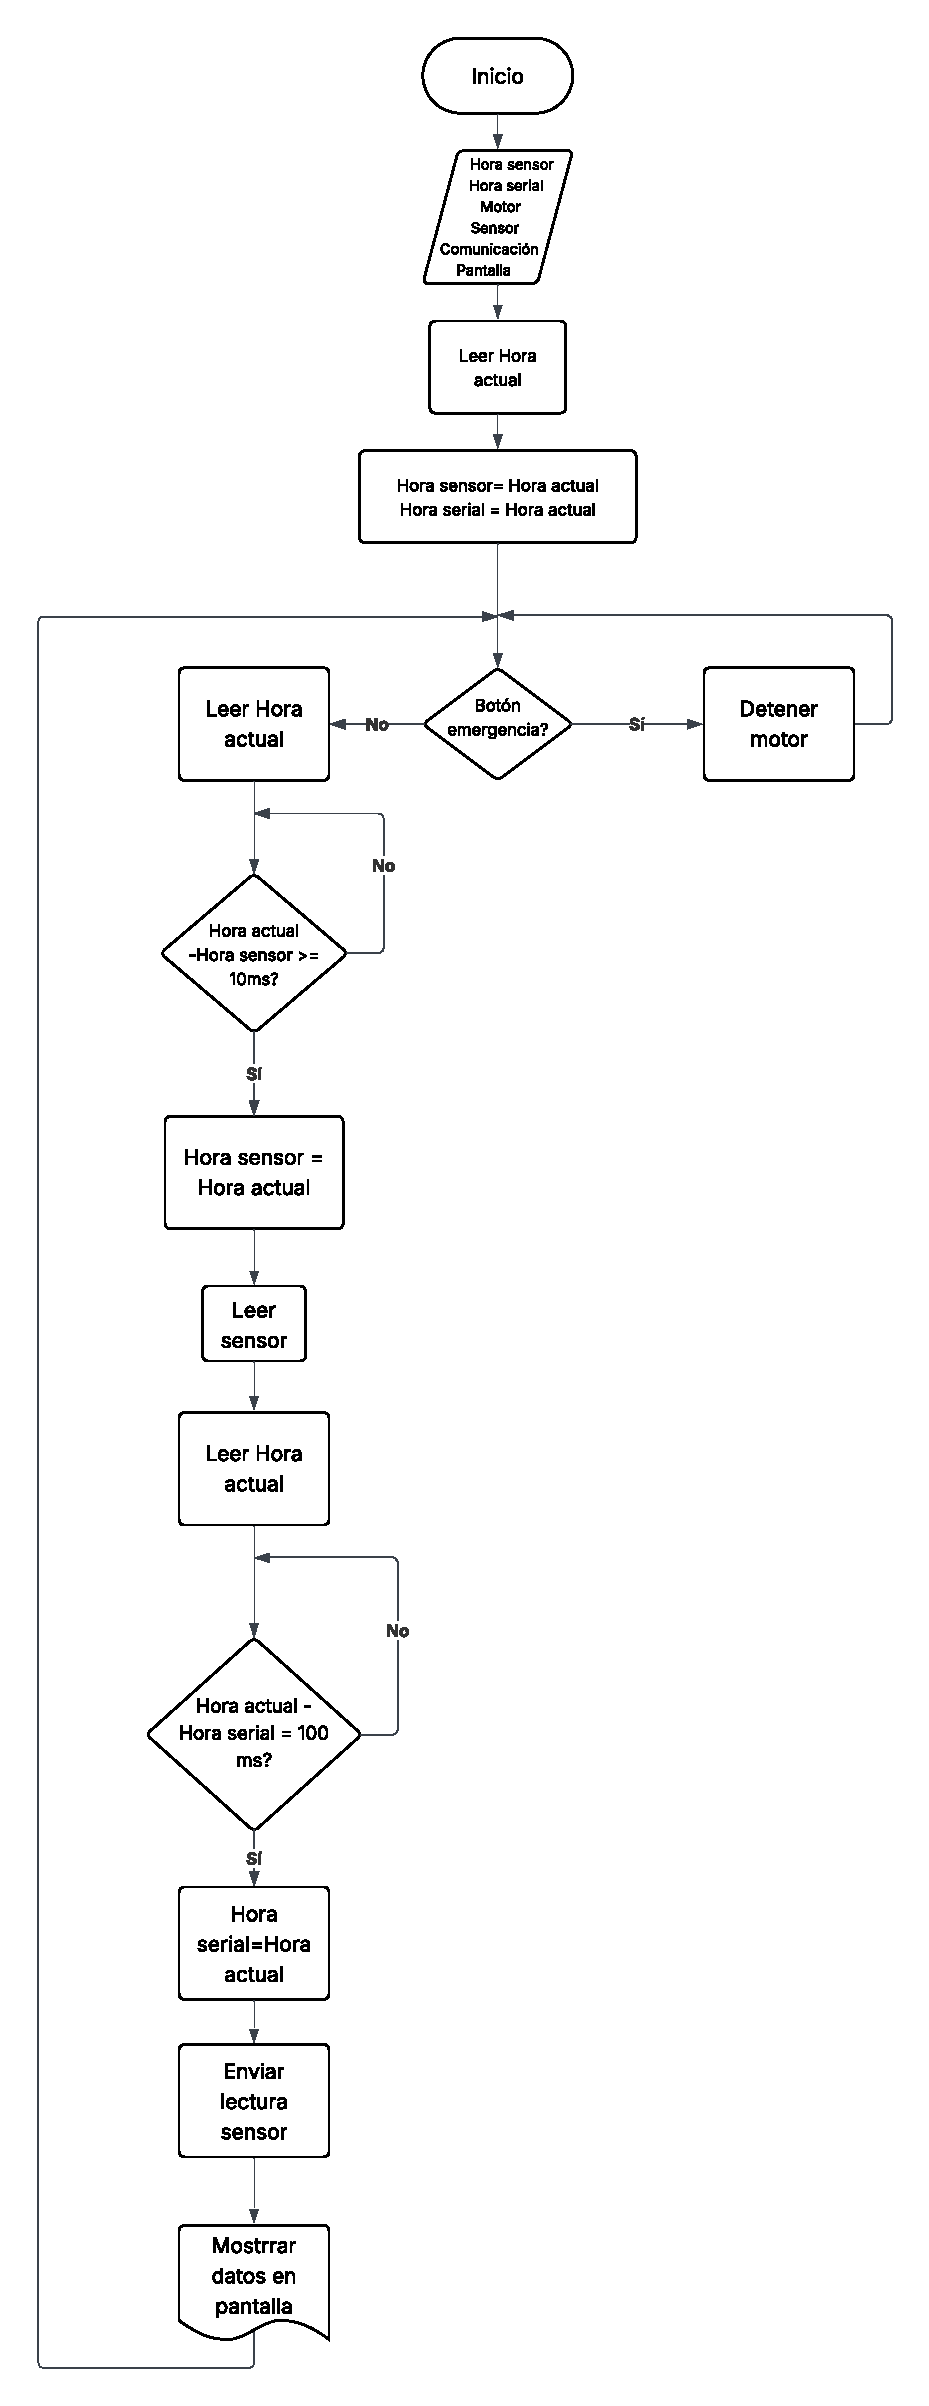
\includegraphics[width=0.4\textwidth]{images/Diagramawhile.pdf}
\caption{Diagrama de flujo de la implementación del while} % Texto bajo la figura
  \label{Diagrama de flujo}          % Etiqueta para referenciar con \ref{fig:res_fig}
\end{figure}
\vspace{0.3cm}
\subsubsection{Trabajo de consulta}
\begin{itemize}
    \item \textbf{Interrupciones:} Las interrupciones son mecanismos que permiten a un microcontrolador suspender temporalmente la ejecución del programa para atender un evento inmediato. Cuando ocurre dicho evento, el hardware guarda el estado del procesador, ejecuta una Rutina de Servicio de Interrupción (\textit{Interrupt Service Routine}-ISR) y luego restaura el estado para continuar la ejecución normal.\\
    Su función principal es evitar el \textit{polling} (método en el que el procesador revisa continuamente si ocurrió un evento, en lugar de esperar a que una interrupción lo notifique) constante y mejorar el tiempo de respuesta ante eventos internos o externos, siendo esenciales en sistemas de tiempo real. \cite{valvano2011embedded} No obstante, pueden generar condiciones de carrera, aumento de latencia si la ISR es extensa y problemas de memoria de pila, por lo que deben implementarse de forma breve y controlada. \cite{buttazzo1997hard}   
    \vspace{0.3cm}
    \item \textbf{Planificación y Scheduler:}  El scheduler (planificador) es el componente del sistema operativo o del software de control que decide qué tarea se ejecuta y en qué momento. En sistemas embebidos con multitarea, su función es administrar el uso del procesador cuando existen varias tareas que requieren ejecución, garantizando orden y control en el acceso al CPU (\textit{Central Processing Unit}).\cite{buttazzo1997hard}
    La prioridad es el nivel de importancia asignado a cada tarea. Determina cuál debe ejecutarse primero cuando varias están listas al mismo tiempo... Una tarea con mayor prioridad desplaza a otra de menor prioridad si el sistema lo permite.
    La planificación preventiva (preemptiva) es aquella en la que el scheduler puede interrumpir una tarea en ejecución para asignar el procesador a otra de mayor prioridad. En cambio, la planificación cooperativa requiere que la tarea en ejecución ceda voluntariamente el control del procesador, por lo que el cambio de tarea ocurre solo cuando esta finaliza o libera el CPU. \cite{buttazzo1997hard}
    \vspace{0.3cm}
    \item \textbf{Multitarea:} La concurrencia es la capacidad de un sistema para gestionar múltiples tareas que progresan en intervalos de tiempo superpuestos. No implica necesariamente que todas se ejecuten exactamente al mismo tiempo, sino que el sistema organiza su ejecución de manera que todas avancen sin bloquearse mutuamente.\cite{buttazzo1997hard}
    La multitarea real ocurre cuando varias tareas se ejecutan simultáneamente en diferentes núcleos de procesamiento. En cambio, la multitarea simulada se presenta en sistemas con un solo núcleo, donde el procesador alterna rápidamente entre tareas mediante un scheduler, dando la impresión de ejecución simultánea aunque solo una tarea se ejecuta en cada instante.\\
    En sistemas embebidos, ejemplos de multitarea incluyen: un microcontrolador que controla un motor mientras lee sensores y transmite datos por comunicación serial; un sistema IoT (\textit{Internet of Things}) que adquiere datos, los procesa y los envía a la nube; o un dispositivo médico que monitorea señales mientras actualiza una pantalla. En todos estos casos, las tareas comparten el procesador y requieren coordinación adecuada. \cite{valvano2011embedded}
     \vspace{0.3cm}
    \item \textbf{Sincronización: } Una condición de carrera es una situación que ocurre cuando dos o más tareas acceden y modifican un mismo recurso o variable compartida de manera simultánea, y el resultado final depende del orden impredecible en que se ejecuten \cite{buttazzo1997hard}. Esto puede generar inconsistencias o corrupción de datos si no existen mecanismos de control adecuados.\\
    Los semáforos y los mutex son mecanismos de sincronización utilizados para coordinar el acceso a recursos compartidos. Un semáforo es una variable de control que regula la disponibilidad de un recurso y puede permitir uno o varios accesos según su tipo. Un mutex (mutual exclusion) es un mecanismo específico que garantiza que solo una tarea a la vez pueda acceder a un recurso, asegurando exclusión mutua.\\
    Una sección crítica es el fragmento de código en el que se accede a un recurso compartido y que, por lo tanto, debe ejecutarse de forma exclusiva para evitar interferencias entre tareas. Para protegerla, se emplean mecanismos como mutex, semáforos o des-habilitación temporal de interrupciones. \cite{valvano2011embedded}
\end{itemize}

\input{tables/table1a.tex}   % Inserta el archivo de tabla (lista de equipos) en este punto




\section{Practicas}\label{sec:metodologia}
  % Metodología: incluye fórmulas, algoritmos o diagrama de flujo.

\subsection{\textbf{Reto 1}} % Sub-sección metodológica
Diseñar un sistema que permita activar una cerradura electrónica si se cumple una condición lógica (contraseña digital o combinación de botones). Requisitos obligatorios:
\begin{itemize}
    \item Entrada digital (botones o teclado)
    \item Salida: LED indicador + actuador (servo o relé)
    \item Manejo de intentos fallidos
    \item Temporizador de bloqueo tras múltiples errores
    \item Modelado opcional como máquina de estados
\end{itemize}
\vspace{0,3cm}
\subsubsection{\textbf{Análisis del problema}}
\begin{itemize}
    \item \textbf{\textit{Identificación de entradas y salidas:}} Según los requisitos obligatorios del sistema, se identifica la necesidad de tener una entrada digital correspondiente, en este caso; a tres botones que ejecutarán la secuencia combinacional para la apertura de la cerradura. En lo que corresponde a la salida, se usa un Diodo LED como indicador lumínico de apertura de la cerradura que será representada por el funcionamiento de un servomotor. 
    \item \textbf{\textit{Restricciones técnicas:}} El sistema presenta restricciones eléctricas relacionadas con los niveles de tensión, corriente máxima de los pines GPIO y los requerimientos de alimentación del actuador.
    \begin{itemize}
        \item El sistema presenta unos limites eléctricos correspondientes a sus 3 elementos principales, ESP32, Servomotor y Led. El microcontrolador ESP32 opera con niveles logicos de 3.3[V] en sus pines GPIO que pueden suministrar corrientes limitadas (12 mA recomendados \cite{espressif2021esp32}) . El servomotor requiere una alimentación de aproximadamente 5[V] y puede generar picos de corriente durante su operación \cite{wahid2024compact}. El LED necesita una resistencia limitadora para controlar y así mismo evitar el sobre consumo.
        \item El sistema debe controlar tiempos específicos, como la duración de apertura del servo y el periodo de bloqueo tras múltiples intentos fallidos. Por lo tanto, el funcionamiento depende de una gestión precisa del tiempo para garantizar un comportamiento adecuado.
        \item Las entradas mediante pulsadores pueden presentar rebote mecánico, lo que puede provocar lecturas inestables si no se considera esta condición en el comportamiento del sistema.
    \end{itemize}
    \item \textbf{\textit{Variables Involucradas:}} Para la implementación del algoritmo de control se definen diversas variables que permiten gestionar el funcionamiento del sistema. Entre ellas se encuentra un arreglo que almacena la contraseña correcta, otro arreglo que almacena la combinación ingresada por el usuario, una variable entera que registra el número de intentos fallidos y una constante que define el número máximo permitido antes de activar el bloqueo. Adicionalmente, se utilizan variables booleanas para indicar si el sistema se encuentra bloqueado y variables relacionadas con temporización para controlar la duración del bloqueo.
\end{itemize}

\subsubsection{\textbf{Flujograma del sistema}}
Se encuentra en la figura \ref{Flujograma reto 1}
\begin{figure}
\centering
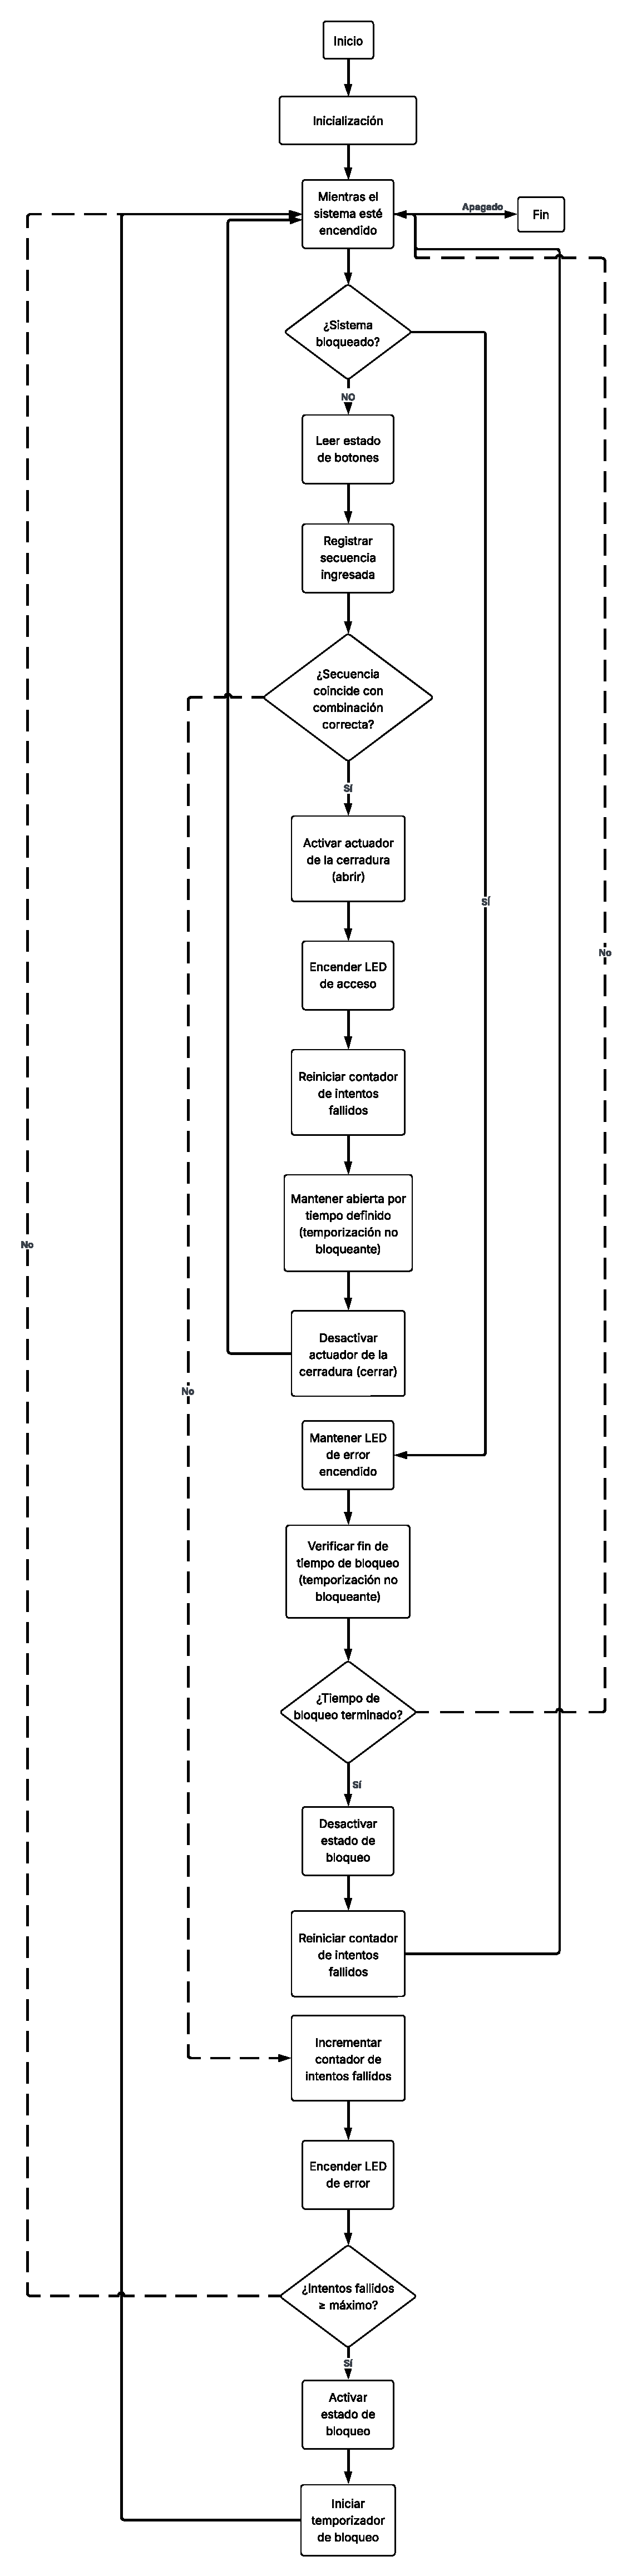
\includegraphics[width=0.3\textwidth]{images/Diagrama en blanco (3).pdf}
\caption{Flujograma reto 1} % Texto bajo la figura
  \label{Flujograma reto 1}          % Etiqueta para referenciar con \ref{fig:res_fig}
\end{figure}
\subsubsection{\textbf{Justificación técnica del microcontrolador seleccionado}}
\vspace{0,3cm}
\begin{itemize}
    \item \textbf{\textit{Número de pines requeridos:}}
    El sistema requiere tres pines de entrada digital para los botones utilizados en la combinación de acceso. Adicionalmente, se requieren dos pines de salida para los LED indicadores de estado (acceso autorizado y acceso denegado) y un pin de salida adicional para el control del actuador de la cerradura (servo motor o relé). En total se requieren aproximadamente seis pines GPIO. El ESP32 dispone de más de 30 pines de entrada/salida programables, por lo que cumple ampliamente con este requerimiento.

    \item \textbf{\textit{Capacidad de procesamiento:}}
    El microcontrolador cuenta con un procesador de doble núcleo basado en arquitectura Tensilica LX6 con frecuencia de operación de hasta 240 MHz, lo cual es suficiente para ejecutar la lógica de control del sistema, realizar la lectura de entradas digitales, gestionar temporizadores y generar señales PWM necesarias para el control de actuadores como servomotores. Su memoria RAM interna también permite implementar estructuras de datos para manejo de estados e intentos de autenticación.

    \item \textbf{\textit{Consumo energético:}}
    El ESP32 presenta un consumo aproximado entre 80 mA y 240 mA en modo activo dependiendo de la carga de procesamiento, y puede reducir su consumo a valores del orden de microamperios cuando se utilizan modos de bajo consumo como deep sleep. Esto resulta adecuado para sistemas de control que permanecen largos periodos en estado de espera.

    \item \textbf{Esquema de conexión:}
    Se encuentra en la imagen \ref{Diagrama de conexión reto 1}
\begin{figure}[H]
\centering
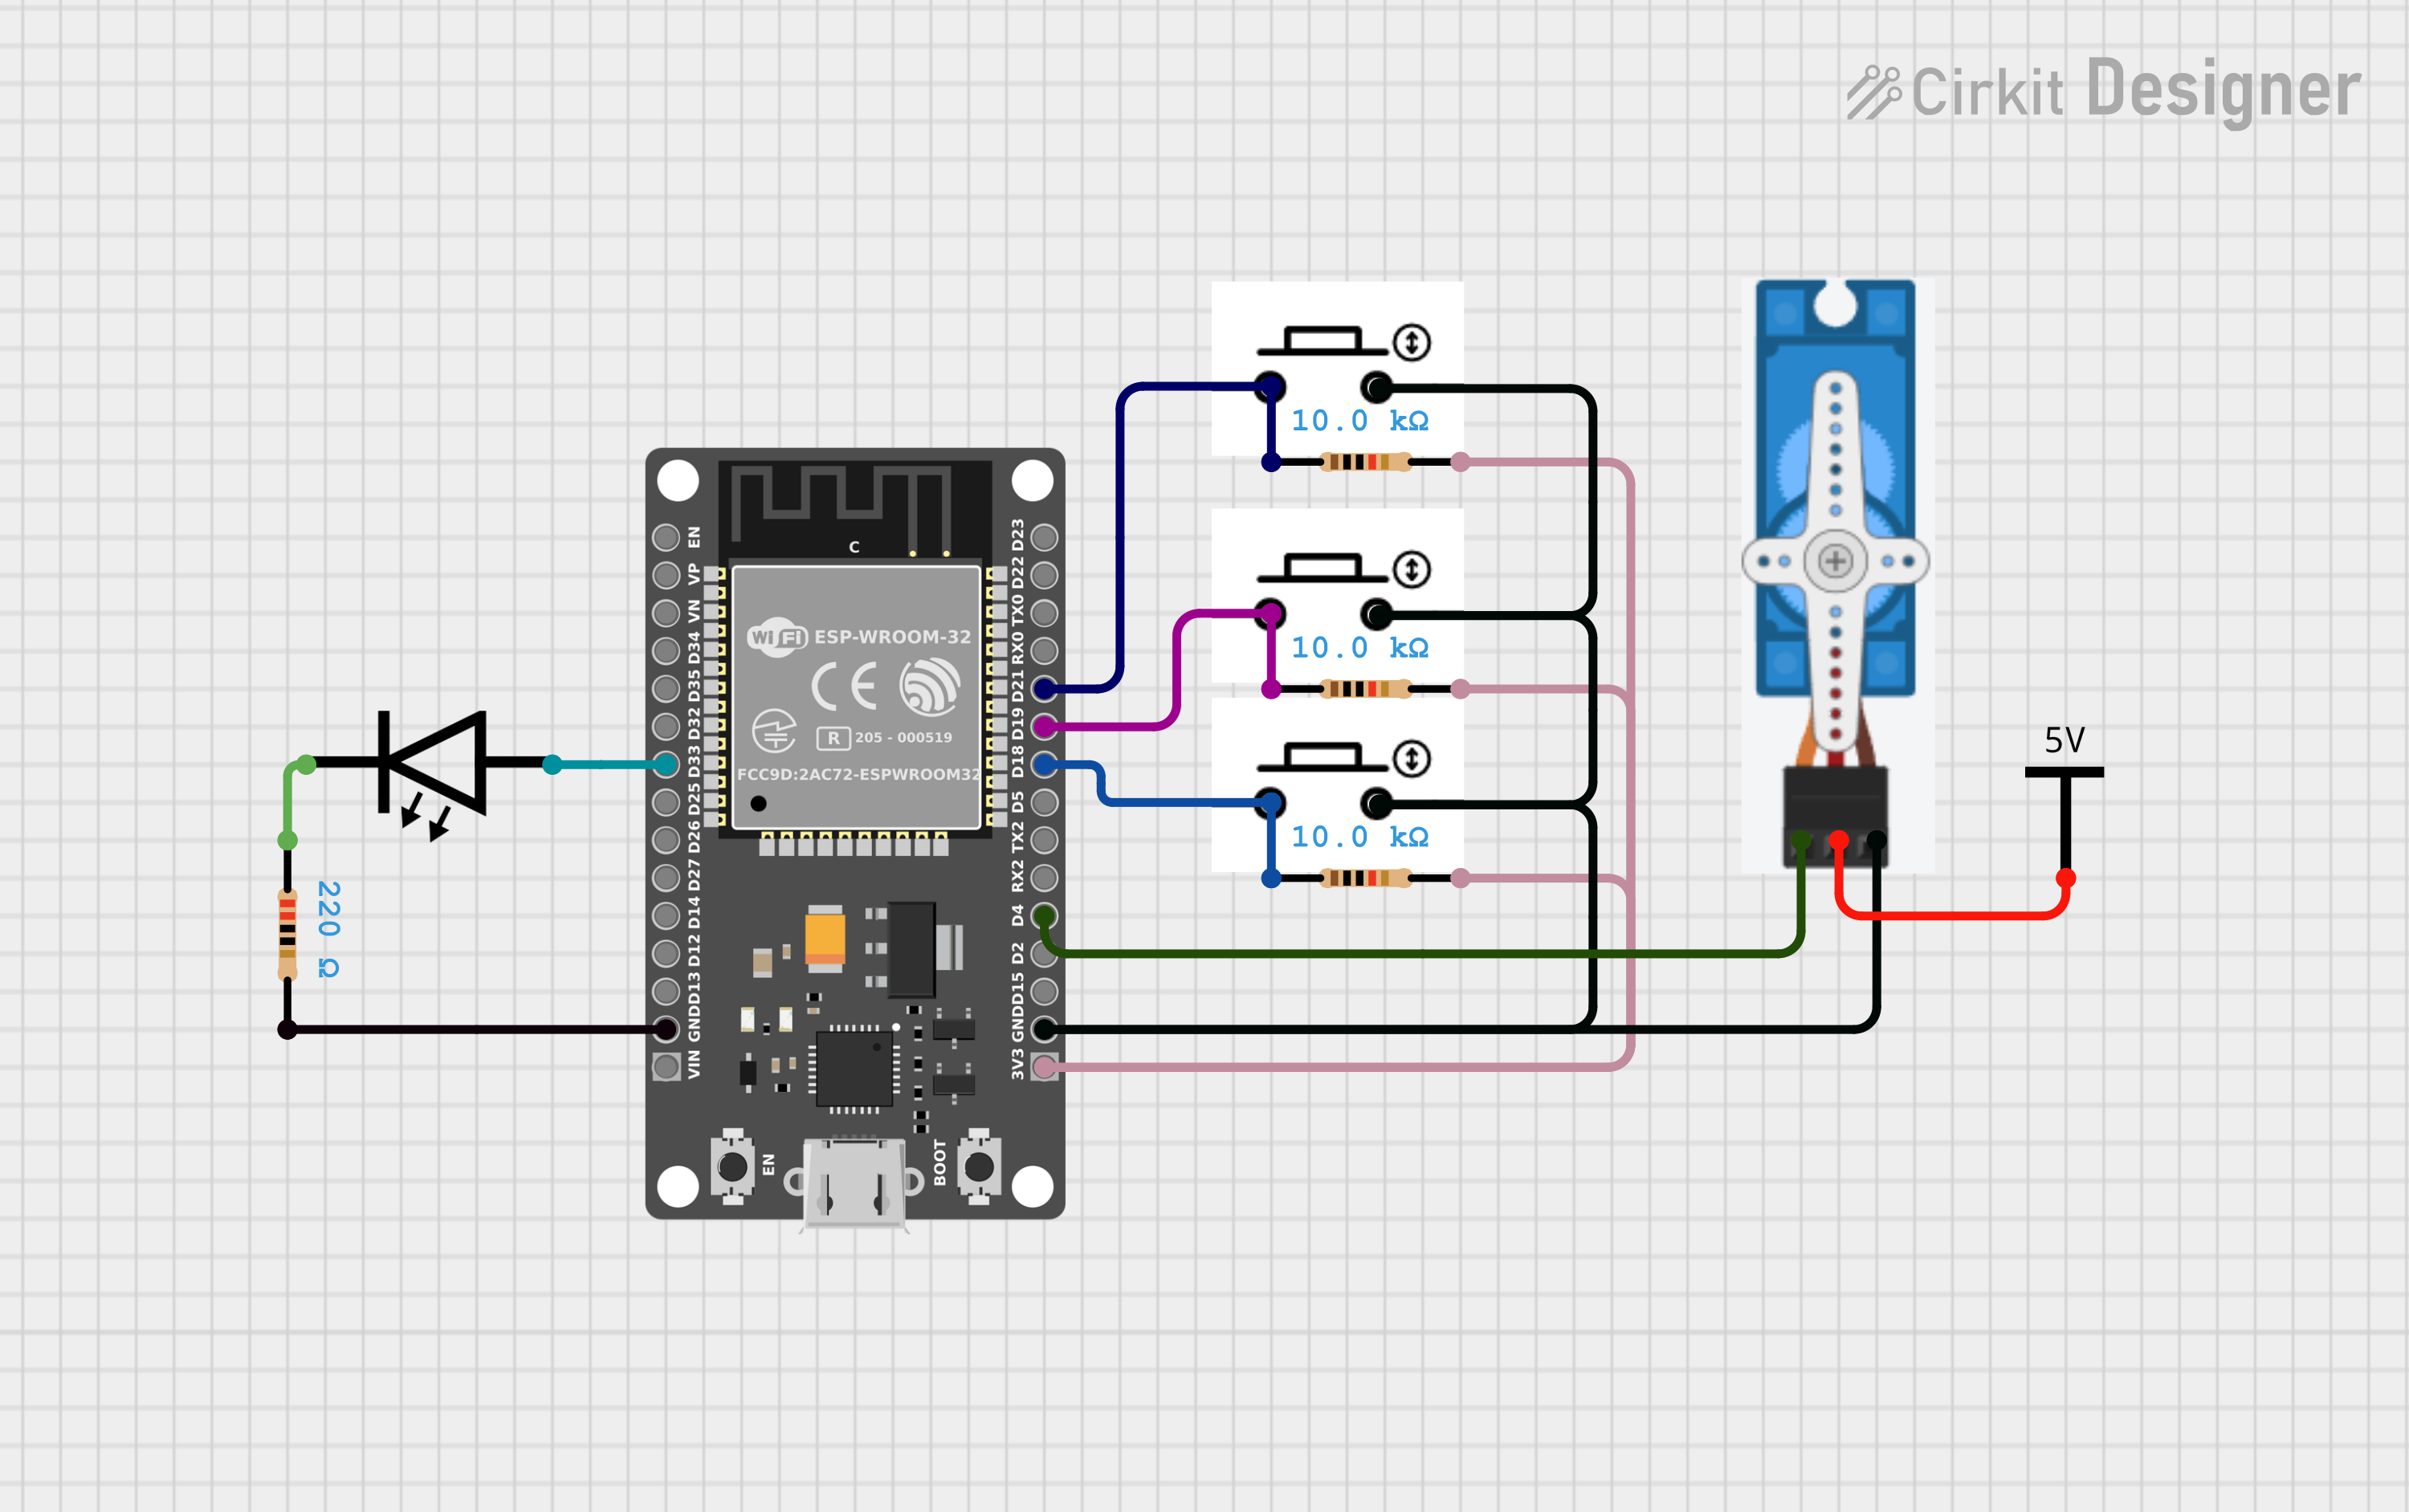
\includegraphics[width=0.4\textwidth]{images/Reto1.png}
\caption{Diagrama de conexión reto 1} % Texto bajo la figura
  \label{Diagrama de conexión reto 1}          % Etiqueta para referenciar con \ref{fig:res_fig}
\end{figure}

    \item \textbf{Componentes auxiliares}
    Para el correcto funcionamiento del sistema se requieren resistencias limitadoras de corriente para los LED (típicamente de 220 Ohm a 330 Ohm), resistencias de polarización para los botones (aproximadamente 10 kOhm), una fuente de alimentación estable para el microcontrolador y el actuador, y en caso de utilizar relé, un transistor driver con diodo de protección para evitar daños por voltajes inducidos. Estos componentes garantizan estabilidad eléctrica, protección de los dispositivos y operación confiable del sistema.
\end{itemize}
\subsubsection{\textbf{Código documentado}}
El código respectivo se encuentra en el anexo \ref{anexo:codigo1}

\subsection{\textbf{Reto 2}} % Sub-sección metodológica
Desarrollar un sistema que supervise una variable física y active alarmas según tres niveles de operación: normal, advertencia y crítico. Requisitos obligatorios:
\begin{itemize}
    \item Definición clara de umbrales
    \item Implementación de histéresis para evitar inestabilidad
    \item Indicadores visuales o sonoros
\end{itemize}
\vspace{0,3cm}
\subsubsection{\textbf{Análisis del problema}}
\begin{itemize}
    \item \textbf{\textit{Identificación de entradas y salidas:}} El sistema requiere una entrada correspondiente a la medición de una variable física que permita evaluar el estado del entorno supervisado. Para efectos de este diseño se selecciona la temperatura como variable de monitoreo, ya que constituye una de las variables más comunes en procesos industriales, sistemas electrónicos y aplicaciones de supervisión ambiental.

    La medición de la temperatura será realizada mediante un sensor de temperatura analógico, el cual entrega una señal proporcional a la magnitud física medida. Esta señal será adquirida por el microcontrolador a través de uno de sus canales de conversión analógico–digital (ADC), permitiendo así transformar la señal analógica en un valor digital interpretable por el sistema.

    En lo que corresponde a las salidas, el sistema contará con indicadores visuales y sonoros que permitirán identificar el estado operativo del sistema de monitoreo. Para ello se emplearán tres diodos LED que representarán los estados de operación normal, advertencia y condición crítica respectivamente. De manera adicional se incorporará una alarma sonora mediante un buzzer, el cual se activará únicamente cuando el sistema detecte que la variable monitoreada ha alcanzado el nivel crítico. 
\vspace{0,3cm}
    \item \textbf{\textit{Restricciones técnicas: }}
    \begin{itemize}
        \item El sensor de temperatura seleccionado entrega una señal analógica que debe ser interpretada por el microcontrolador \cite{LM35_datasheet}. Por lo tanto, el dispositivo de procesamiento debe contar con un convertidor analógico–digital con suficiente resolución para permitir una medición adecuada de la variable física.
        \item Los diodos LED empleados como indicadores visuales requieren la inclusión de resistencias limitadoras de corriente, ya que los pines GPIO del microcontrolador presentan límites de corriente que no deben ser superados para evitar daños en el dispositivo.
        \item En el caso del buzzer o alarma sonora, es necesario considerar que algunos dispositivos pueden requerir corrientes superiores a las que puede suministrar directamente un pin del microcontrolador\cite{buzzer_datasheet}. En estas condiciones puede ser necesario incorporar una etapa de conmutación basada en transistor, que permita manejar la carga sin comprometer la integridad del microcontrolador.
        \item Una restricción fundamental en este tipo de sistemas corresponde a la inestabilidad que puede presentarse cerca de los umbrales de decisión. Cuando la variable medida se encuentra próxima al valor límite entre dos estados, pequeñas fluctuaciones pueden provocar cambios continuos entre estados consecutivos. Para evitar este comportamiento se implementa un mecanismo de histéresis, el cual introduce un margen de diferencia entre los valores de activación y desactivación de cada estado \cite{temperature_hysteresis_cadence}.
    \end{itemize}
    \item 
    \textbf{\textit{Variables Involucradas:}}Variable que almacena el valor digital leído del convertidor analógico–digital correspondiente al sensor de temperatura. Variables que definen los umbrales del sistema para los estados normal, advertencia y crítico. Variable que indica el estado actual del sistema para activar los indicadores correspondientes. Variable que establece el margen de histéresis para evitar cambios repetitivos entre estados. Variables auxiliares para controlar el tiempo de muestreo y la frecuencia de lectura del sensor.
\end{itemize}

\subsubsection{\textbf{Flujograma del sistema}}
Se encuentra en la figura \ref{Flujograma reto 2}.
\begin{figure}
\centering
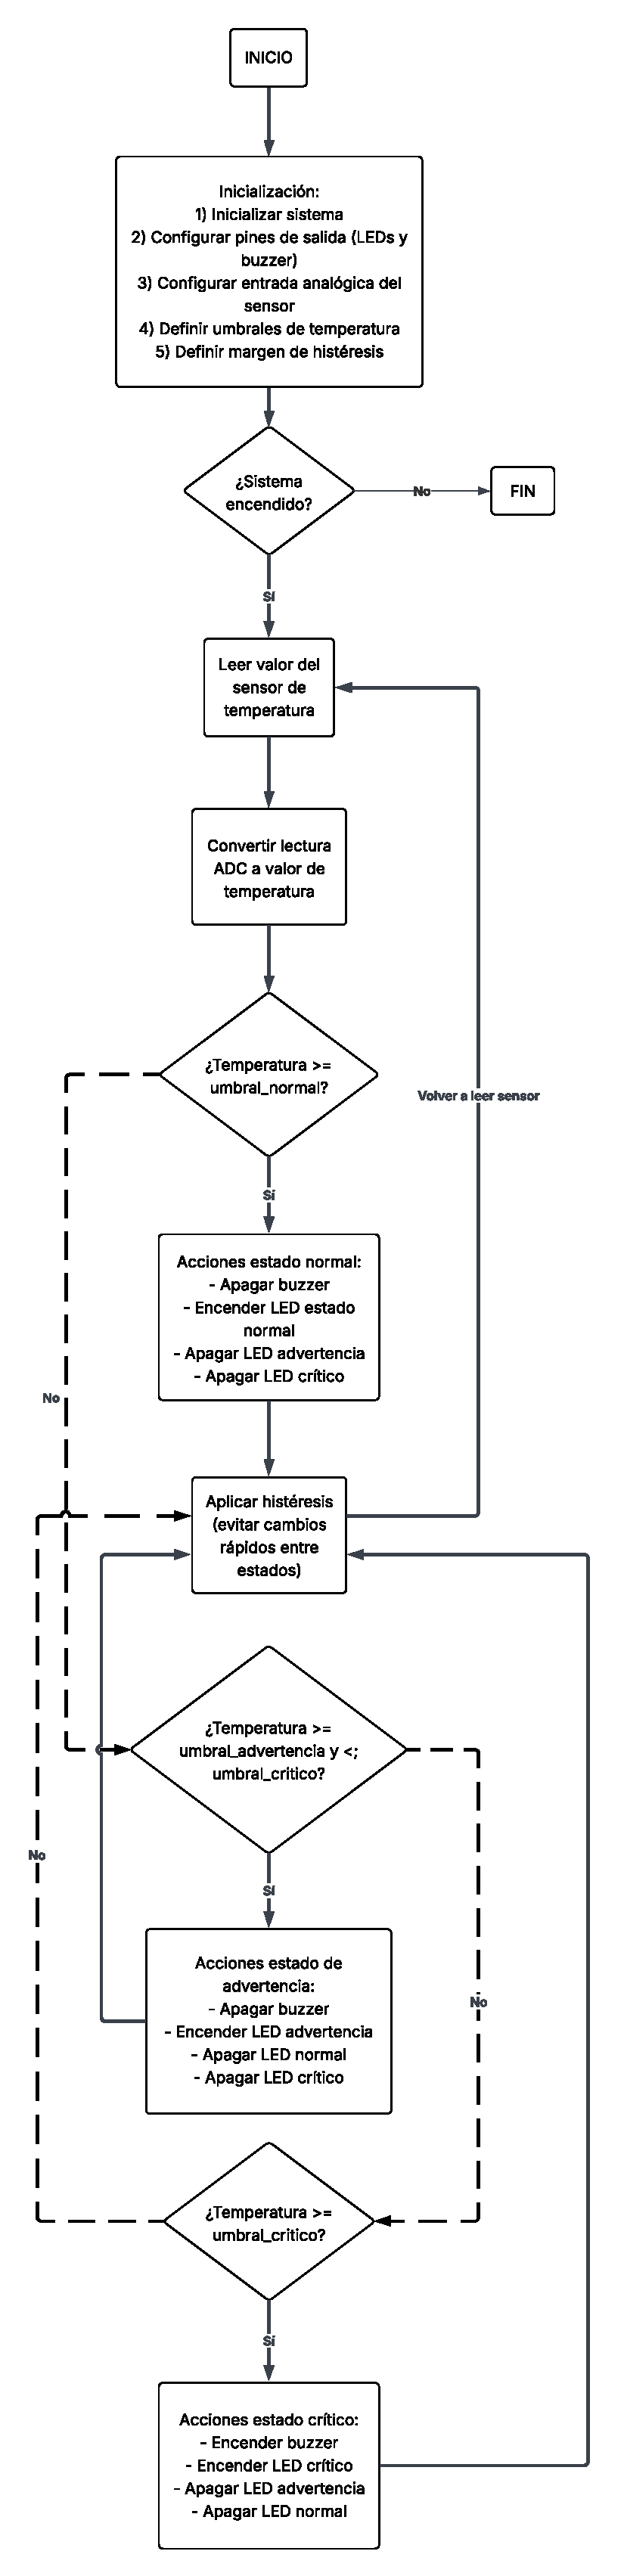
\includegraphics[width=0.3\textwidth]{images/Diagrama en blanco (1).pdf}
\caption{Flujograma reto 2} % Texto bajo la figura
  \label{Flujograma reto 2}          % Etiqueta para referenciar con \ref{fig:res_fig}
\end{figure}
\subsubsection{\textbf{Justificación técnica del microcontrolador seleccionado}}
\begin{itemize}
    \item \textbf{\textit{Número de pines requeridos.}}
    El sistema requiere al menos un pin de entrada analógica para la lectura del sensor que mide la variable física supervisada. Adicionalmente, se requieren tres pines de salida digital para los indicadores de estado correspondientes a los niveles de operación: normal, advertencia y crítico. También puede incorporarse un pin adicional para activar una alarma sonora mediante un buzzer. En total, el sistema requiere aproximadamente cinco pines de entrada/salida. El microcontrolador ESP32 dispone de múltiples pines GPIO y varios canales ADC de 12 bits \cite{espressif2021esp32}, lo que permite realizar la adquisición de la señal del sensor con suficiente resolución. 

    \item \textbf{\textit{Capacidad de procesamiento.}}
    El ESP32 cuenta con un procesador de doble núcleo con frecuencia de operación de hasta 240 MHz \cite{espressif2021esp32}, lo cual permite ejecutar el algoritmo de monitoreo en tiempo real, realizar la conversión analógica-digital de la señal del sensor y aplicar la lógica de comparación con los umbrales definidos. Además, su capacidad de procesamiento permite implementar histéresis en los niveles de alarma para evitar conmutaciones rápidas e inestables cuando la variable medida se encuentra cercana a los valores límite \cite{espressif2021esp32}.

    \item \textbf{\textit{Consumo energético.}}
    El dispositivo presenta un consumo aproximado entre 80 mA y 240 mA en modo activo, dependiendo de la carga de procesamiento y los periféricos utilizados. Asimismo, dispone de modos de bajo consumo que reducen significativamente la corriente cuando el sistema se encuentra en espera. Esto permite su utilización en sistemas de monitoreo continuo sin requerir un consumo energético elevado.

    \item \textbf{\textit{Esquema de conexión.}}
    Se encuentra en la imagen \ref{Diagrama de conexión reto 2}
\begin{figure}[H]
\centering
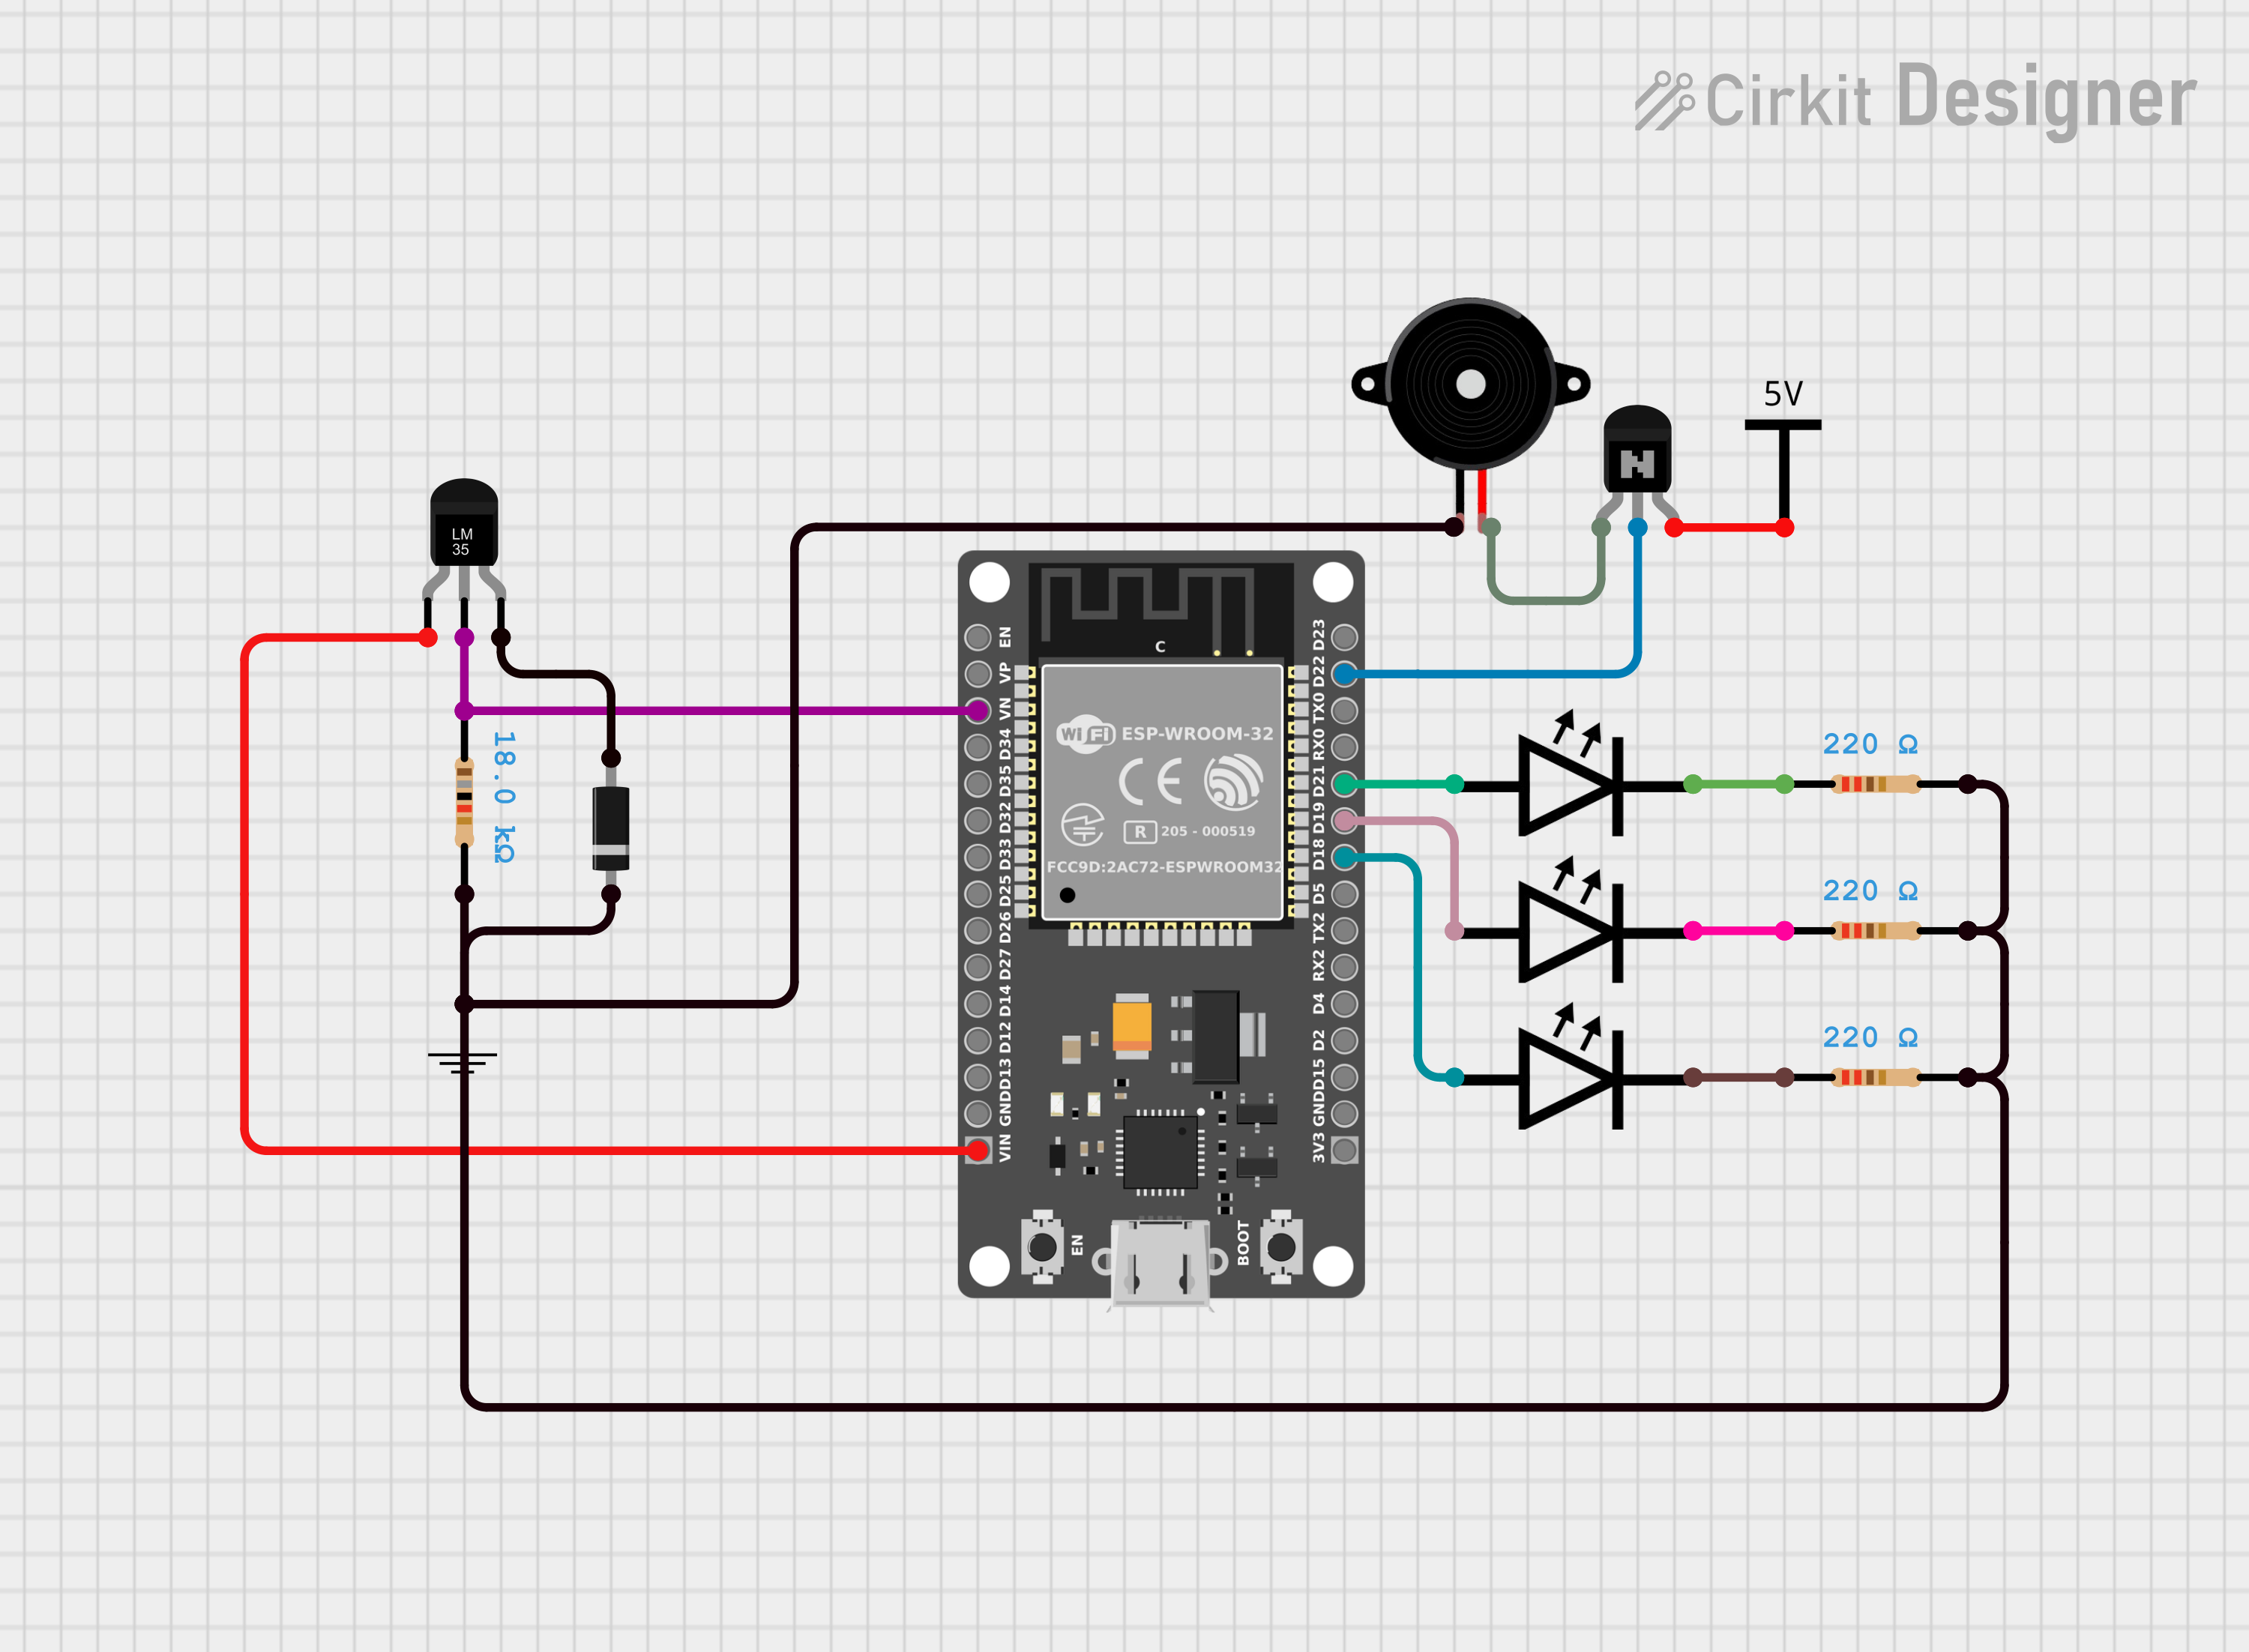
\includegraphics[width=0.4\textwidth]{images/Reto2.png}
\caption{Diagrama de conexión reto 2} % Texto bajo la figura
  \label{Diagrama de conexión reto 2}          % Etiqueta para referenciar con \ref{fig:res_fig}
\end{figure}

    \item \textbf{\textit{Componentes auxiliares}}
    El sistema requiere resistencias limitadoras de corriente para los LED indicadores (220 Ohm a 330 Ohm), resistencias de polarización en caso de utilizar sensores analógicos que lo requieran, y una fuente de alimentación estable para el microcontrolador y los dispositivos de salida. Si se emplea un buzzer activo o una alarma de mayor potencia, puede ser necesario utilizar un transistor driver para manejar la corriente requerida.
\end{itemize}

\subsubsection{\textbf{Código documentado}}
El código respectivo se encuentra en el anexo \ref{anexo:codigo2}

\subsection{\textbf{Reto 3}} % Sub-sección metodológica
Diseñar un sistema de riego automático para cultivo de tomate. El sistema debe: 
Monitorear la humedad del suelo,  
Activar riego cuando la humedad esté por debajo de un umbral, 
Detener el riego cuando se alcance nivel adecuado, 
Evitar inestabilidad mediante histéresis,  
Funcionar como sistema secuencial autónomo e  
Implemente temporización no bloqueante.


\subsubsection{\textbf{Análisis del problema}}
\begin{itemize}
    \item \textbf{\textit{Identificación de entradas y salidas:}}
    La entrada principal es un sensor de humedad del suelo conectado a una entrada analógica del microcontrolador. La salida corresponde al actuador de riego (bomba o válvula solenoide) controlado mediante un relé o transistor de potencia. Opcionalmente se puede incluir un LED indicador de estado del sistema.

    \item \textbf{\textit{Restricciones técnicas:}}
    \begin{itemize}
        \item El microcontrolador debe disponer de al menos una entrada analógica (ADC) para la lectura del sensor de humedad.

        \item Debe existir una salida digital capaz de controlar un relé o transistor para activar la bomba o válvula de riego.

        \item El sistema debe operar con niveles de voltaje compatibles (3.3 V o 5 V) entre microcontrolador, sensor y etapa de potencia. \cite{espressif2021esp32}

        \item El control del riego debe implementar histéresis mediante dos umbrales de humedad para evitar conmutaciones rápidas.

        \item El software debe emplear temporización no bloqueante (por ejemplo mediante contadores de tiempo) para permitir lecturas periódicas del sensor.

    \end{itemize}

    \item \textbf{\textit{Variables involucradas:}}
    Las variables principales son el valor de humedad del suelo medido por el sensor, el umbral inferior de activación del riego, el umbral superior de desactivación, el estado del sistema (riego activo o inactivo) y las variables de temporización utilizadas para el muestreo periódico del sensor.
\end{itemize}

\subsubsection{\textbf{Flujograma del sistema} }
Se encuentra en la figura \ref{Flujograma reto 3}
\begin{figure}
\centering
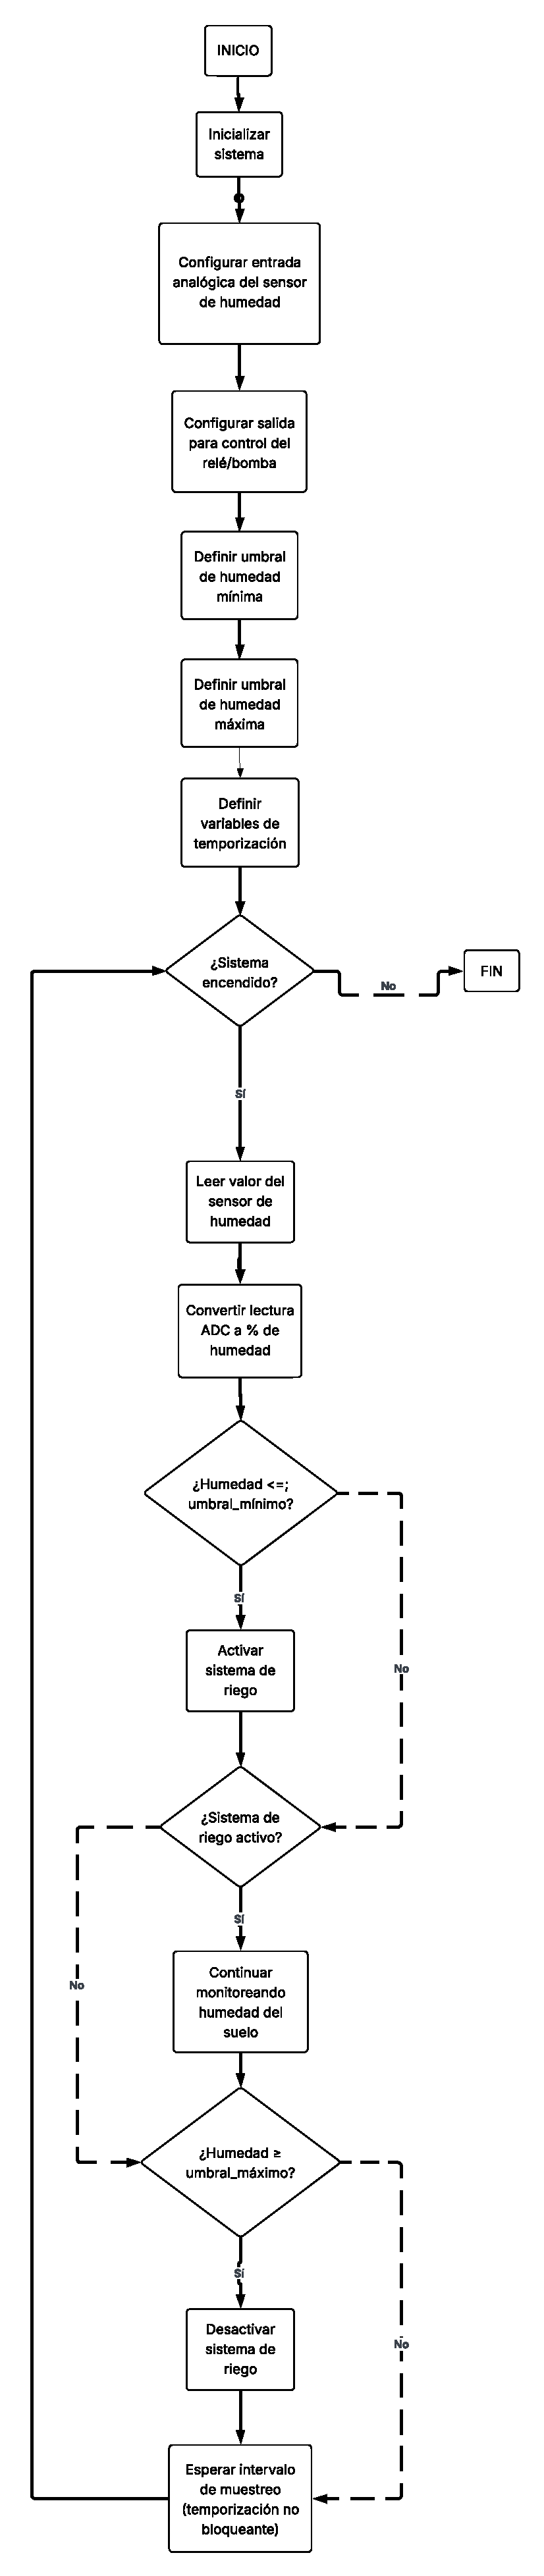
\includegraphics[width=0.25\textwidth]{images/Diagrama en blanco (2).pdf}
\caption{Flujograma reto 3} % Texto bajo la figura
  \label{Flujograma reto 3}          % Etiqueta para referenciar con \ref{fig:res_fig}
\end{figure}
\subsubsection{\textbf{Justificación técnica del microcontrolador seleccionado}}
\begin{itemize}
    \item \textbf{\textit{Número de pines requeridos:}}
    El sistema requiere 1 entrada analógica para el sensor de humedad del suelo y 1 salida digital para controlar el relé o transistor que activa la bomba de riego. Opcionalmente se puede utilizar 1 salida digital adicional para un LED indicador. El ESP32 dispone de más de 30 pines GPIO, incluyendo múltiples entradas ADC, por lo que satisface ampliamente los requerimientos del sistema. 

    \item \textbf{\textit{Capacidad de procesamiento:}}
    El ESP32 integra un procesador dual-core de hasta 240 MHz \cite{espressif2021esp32}, suficiente para ejecutar el algoritmo de control secuencial, realizar lecturas periódicas del sensor mediante ADC, aplicar histéresis entre umbrales de humedad y gestionar temporización no bloqueante para el monitoreo continuo del sistema.

    \item \textbf{\textit{Consumo energético:}}
    El microcontrolador opera a 3.3 V y presenta un consumo aproximado de 80–240 mA en operación \cite{espressif2021esp32}, con modos de bajo consumo disponibles. Esto permite su integración en sistemas agrícolas automatizados con alimentación estable o mediante fuentes reguladas.

    \item \textbf{\textit{Esquema de conexión (diagrama eléctrico o esquemático):}}
    Se encuentra en la imagen \ref{Diagrama de conexión reto 3}
\begin{figure}[H]
\centering
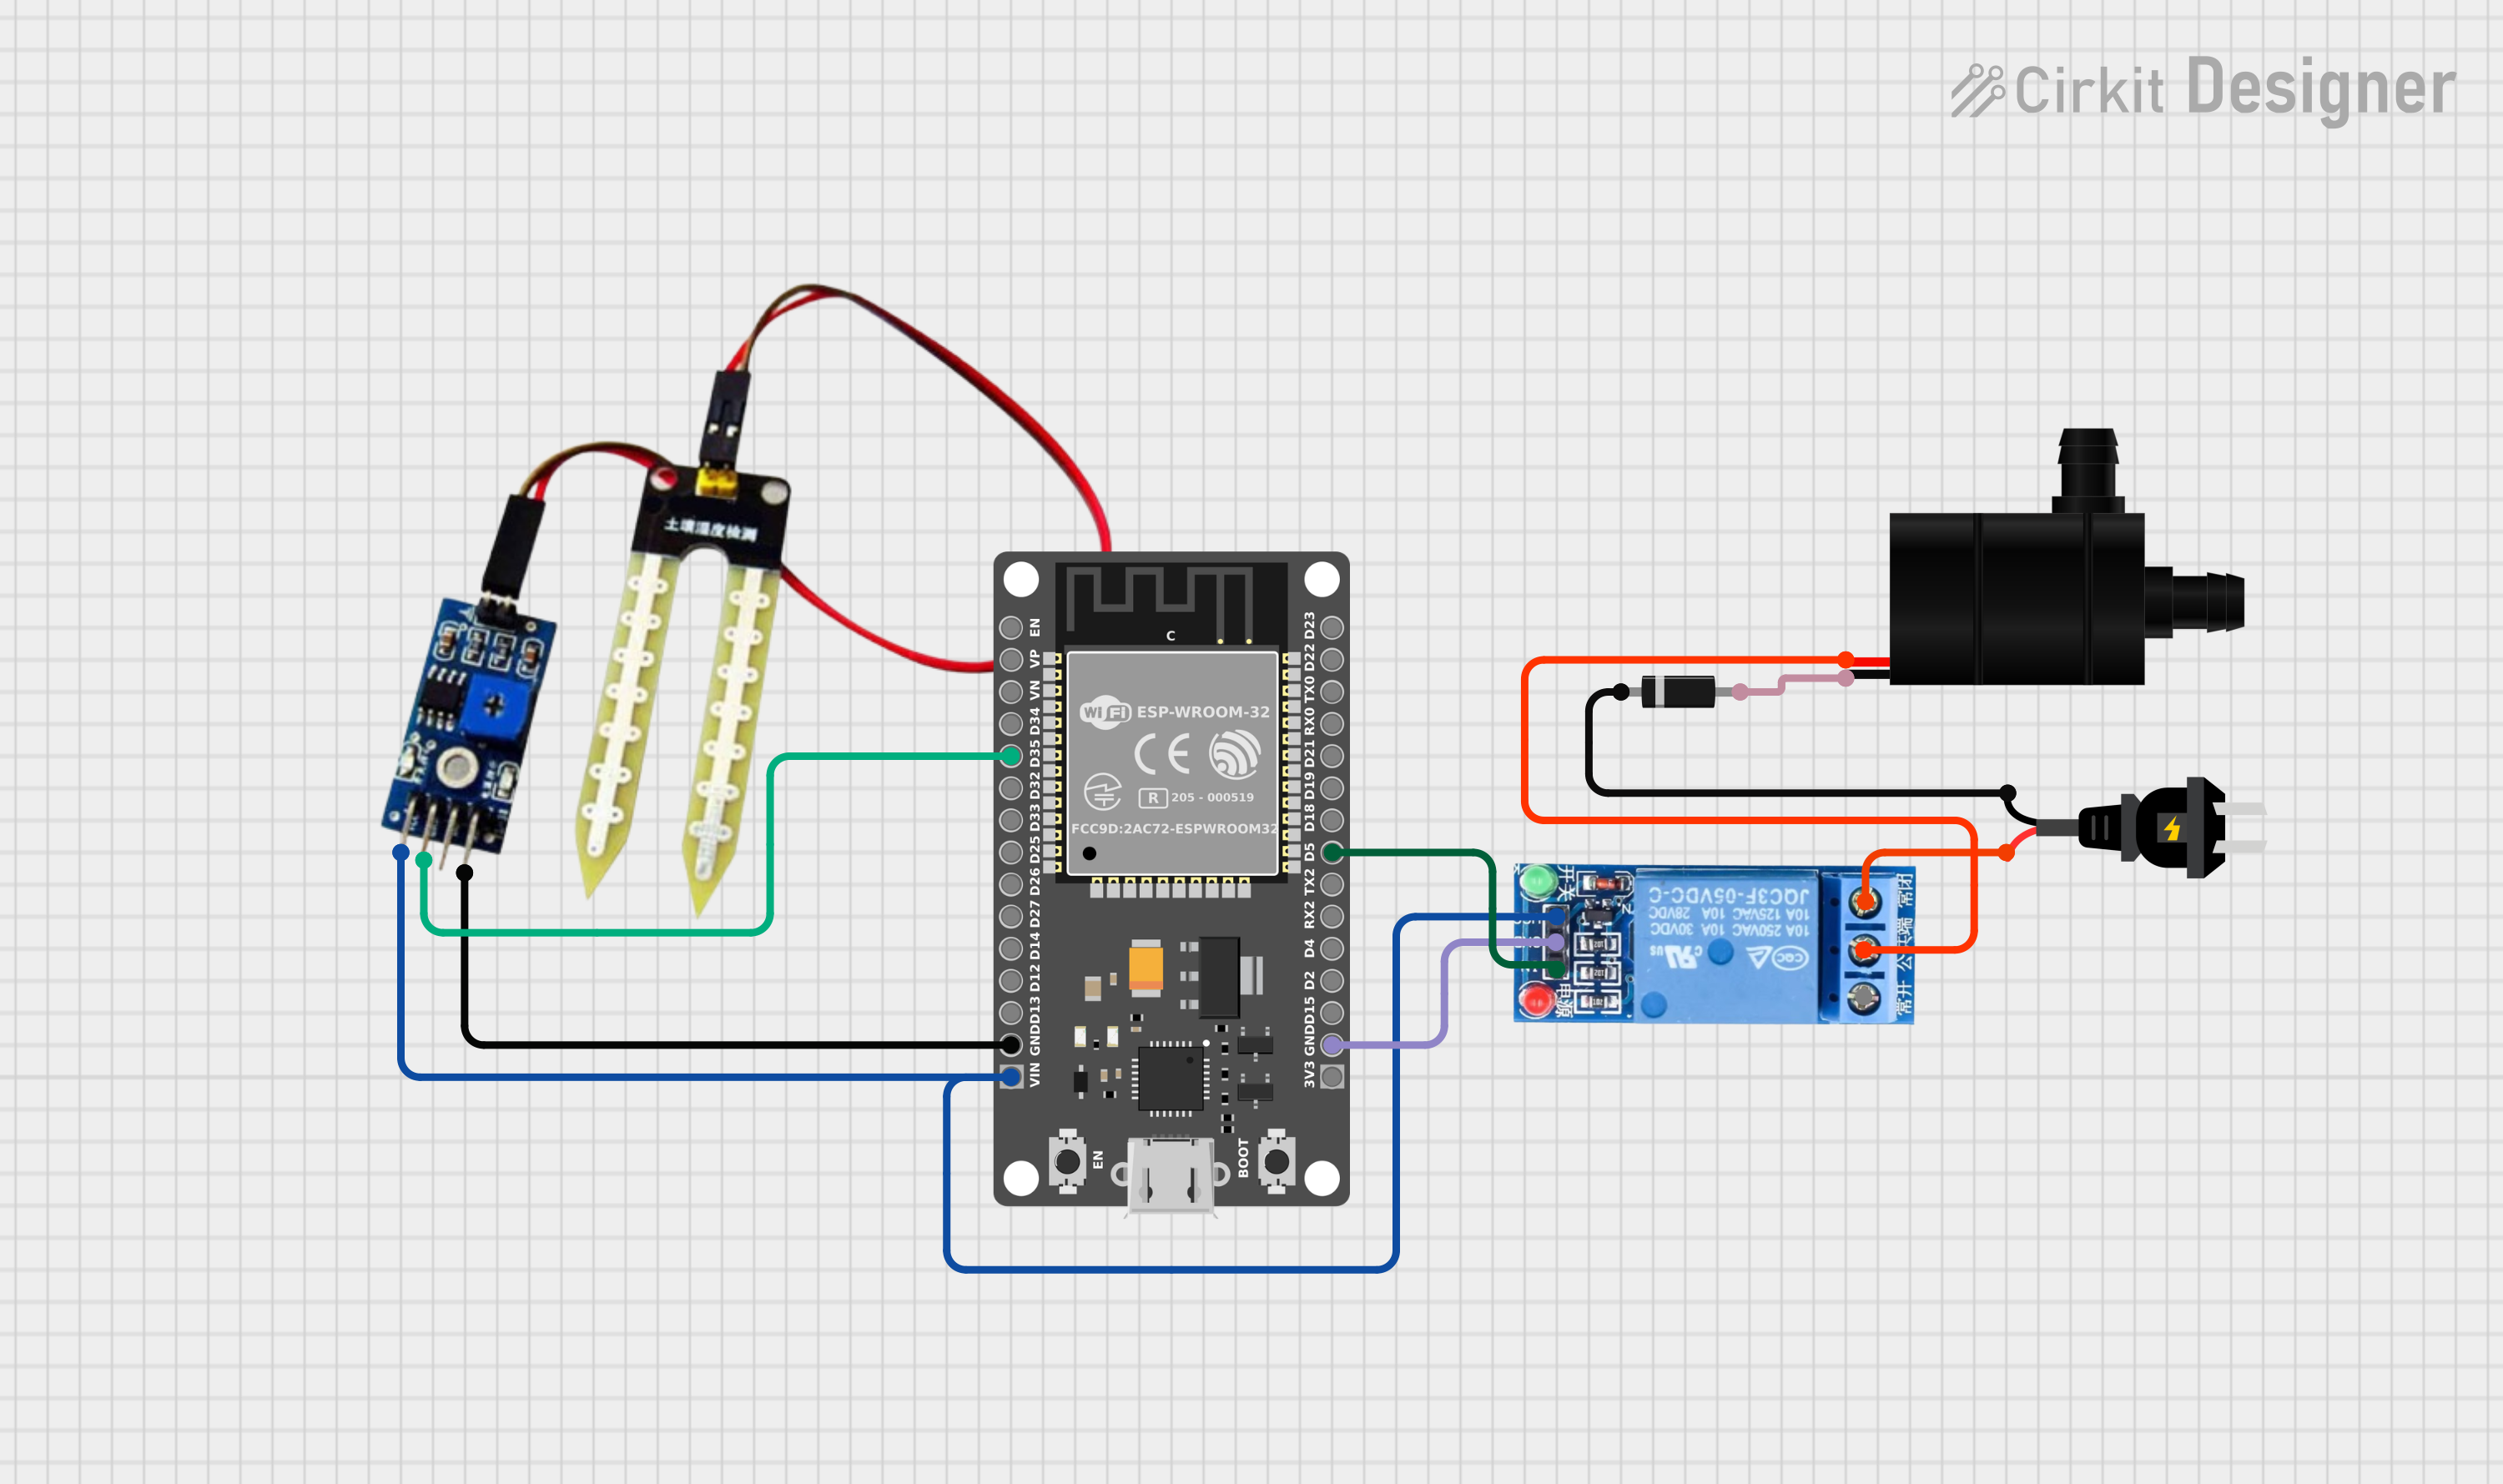
\includegraphics[width=0.4\textwidth]{images/Reto3.png}
\caption{Diagrama de conexión reto 3} % Texto bajo la figura
  \label{Diagrama de conexión reto 3}          % Etiqueta para referenciar con \ref{fig:res_fig}
\end{figure}

    \item\textbf{\textit{Componentes auxiliares}} El sistema requiere un sensor de humedad del suelo, un módulo relé o MOSFET de potencia, resistencias de polarización para el control del transistor, diodo de protección, una bomba de agua o válvula solenoide para el riego y opcionalmente LEDs indicadores para mostrar el estado del sistema.
\end{itemize}
\subsubsection{\textbf{Código documentado}}
El código respectivo se encuentra en el anexo \ref{anexo:codigo3}



  
\section{Protocolos de comunicación}
Los protocolos de comunicación permiten el intercambio de datos entre dispositivos dentro de un sistema embebido. Estos pueden ser de tipo serial o inalámbrico, dependiendo del medio de transmisión.

\subsection{Comunicación Serial}

La comunicación serial se basa en la transmisión secuencial de datos bit a bit a través de un canal, lo que permite reducir el cableado y mejorar la eficiencia del hardware.

\begin{itemize}
    \item Transmisión secuencial de información
    \item Reducción del cableado
    \item Mayor eficiencia en el diseño
    \item Conexión entre microcontroladores y periféricos
\end{itemize}

Dentro de la comunicación serial se destacan los siguientes protocolos:

\subsubsection{UART (Universal Asynchronous Receiver-Transmitter)}

Es un protocolo de comunicación asíncrono que no utiliza señal de reloj compartida.

\begin{itemize}
    \item Comunicación punto a punto
    \item Uso de tramas de datos
    \item Configuración mediante baudios, bits de datos, paridad y bits de parada
    \item Solo requiere dos líneas: TX y RX (más GND)
\end{itemize}

\textbf{Ventajas:}
\begin{itemize}
    \item Simplicidad
    \item Bajo costo
    \item Comunicación full-duplex
    \item Mayor alcance comparado con otros protocolos seriales
\end{itemize}

\subsubsection{I2C (Inter-Integrated Circuit)}

Es un protocolo síncrono que permite la conexión de múltiples dispositivos utilizando solo dos líneas.

\begin{itemize}
    \item Líneas: SDA (datos) y SCL (reloj)
    \item Permite múltiples dispositivos en el mismo bus
    \item Maneja direccionamiento (7 y 10 bits)
    \item Requiere resistencias pull-up
\end{itemize}

\textbf{Ventajas:}
\begin{itemize}
    \item Reduce el número de conexiones
    \item Facilita la interconexión de varios periféricos
\end{itemize}

\subsubsection{SPI (Serial Peripheral Interface)}

Es un protocolo síncrono de alta velocidad basado en una arquitectura maestro-esclavo.

\begin{itemize}
    \item Líneas: MOSI, MISO, SCK y SS/CS
    \item Comunicación full-duplex
    \item Alta velocidad de transmisión
    \item Sincronización mediante señal de reloj
\end{itemize}

\textbf{Ventajas:}
\begin{itemize}
    \item Alta velocidad
    \item Precisión en la transmisión de datos
\end{itemize}

\subsubsection{Comparación de Protocolos}

\begin{center}
\resizebox{\columnwidth}{!}{
\begin{tabular}{|c|c|c|c|}
\hline
\textbf{Característica} & \textbf{UART} & \textbf{I2C} & \textbf{SPI} \\
\hline
Tipo & Asíncrono & Síncrono & Síncrono \\
\hline
Líneas & TX, RX & SDA, SCL & MOSI, MISO, SCK, SS \\
\hline
Reloj & No & Sí & Sí \\
\hline
Dispositivos & 2 & Múltiples & Maestro-esclavos \\
\hline
Velocidad & Media & Media & Alta \\
\hline
Complejidad & Baja & Media & Media \\
\hline
\end{tabular}
}
\end{center}  

\subsubsection{Criterios de Selección}

\begin{itemize}
    \item Para alta velocidad: SPI
    \item Para múltiples dispositivos con pocas líneas: I2C
    \item Para comunicación simple punto a punto: UART
\end{itemize}

\subsection{Comunicación Inalámbrica}

Los protocolos inalámbricos son fundamentales en aplicaciones IoT y permiten la comunicación sin necesidad de conexiones físicas.

\begin{itemize}
    \item Bluetooth Low Energy (BLE): bajo consumo y corto alcance
    \item Wi-Fi: alta tasa de datos e integración a internet
    \item Zigbee: redes malladas de bajo consumo
    \item Thread: comunicación en malla basada en IPv6
    \item LoRaWAN: largo alcance y bajo consumo
    \item NB-IoT: comunicación celular para IoT
\end{itemize}

\subsubsection{Principales protocolos inalámbricos}

\paragraph{\textbf{WI-Fi}}

Protocolo diseñado inicialmente para redes de computadoras y acceso a internet. Actualmente es ampliamente utilizado en dispositivos IoT con suficiente disponibilidad energética.

\begin{itemize}
    \item Alcance: $\sim$100 m
    \item Velocidad: Alta (hasta Gbps)
    \item Uso: Cámaras, ESP32, interfaces HMI
\end{itemize}

\paragraph{\textbf{Bluetooth y Bluetooth Low Energy (BLE)}}

Bluetooth es un estándar de corto alcance, mientras que BLE está optimizado para bajo consumo energético, ideal para dispositivos alimentados por batería.

\begin{itemize}
    \item Alcance: 10–100 m
    \item Velocidad: Media (1–3 Mbps)
    \item Uso: Wearables, sensores cercanos
\end{itemize}

\paragraph{\textbf{ZigBee}}

Protocolo orientado a redes de sensores distribuidos con bajo consumo energético, utilizando topologías malladas.

\begin{itemize}
    \item Alcance: $\sim$100 m
    \item Velocidad: Baja (250 kbps)
    \item Uso: Domótica, automatización industrial
\end{itemize}

\paragraph{\textbf{Thread}}

Protocolo de red mallada basado en IPv6, diseñado para IoT, con capacidad de auto-reparación y bajo consumo energético.

\begin{itemize}
    \item Red mallada segura
    \item Optimizado para dispositivos de baja potencia
    \item Uso: Hogares inteligentes y edificios
\end{itemize}

\paragraph{\textbf{LoRaWAN}}

Protocolo de largo alcance y bajo consumo, ideal para aplicaciones donde los dispositivos están muy alejados entre sí.

\begin{itemize}
    \item Alcance: 2–15 km
    \item Velocidad: Muy baja
    \item Uso: Agricultura, monitoreo ambiental, ciudades inteligentes
\end{itemize}

\begin{table}[H]
\centering
\begin{tabular}{|c|c|c|c|}
\hline
Tecnología & Alcance & Velocidad & Aplicación \\
\hline
Wi-Fi & $\sim$100 m & Alta & Internet, video, IoT con energía \\
\hline
Bluetooth/BLE & 10–100 m & Media & Sensores, wearables \\
\hline
ZigBee & $\sim$100 m & Baja & Domótica \\
\hline
LoRaWAN & 2–15 km & Muy baja & Monitoreo remoto \\
\hline
\end{tabular}
\caption{Comparación de protocolos inalámbricos}
\end{table}

\subsubsection{Criterios de selección}

La elección del protocolo inalámbrico debe considerar:

\begin{itemize}
    \item \textbf{Alcance:} Distancia entre dispositivos
    \item \textbf{Consumo energético:} Especialmente en dispositivos con batería
    \item \textbf{Velocidad de transmisión:} Cantidad de datos a enviar
    \item \textbf{Aplicación:} Tipo de sistema (industrial, doméstico, urbano)
\end{itemize}

En general:
\begin{itemize}
    \item Wi-Fi: cuando se requiere alta velocidad
    \item BLE: cuando se necesita bajo consumo
    \item ZigBee/Thread: redes de múltiples dispositivos
    \item LoRaWAN: comunicación a larga distancia
\end{itemize}

\subsubsection{Importancia en IoT}

Los protocolos inalámbricos son la base del IoT, ya que permiten conectar sensores, dispositivos y sistemas a internet sin infraestructura cableada. Su correcta selección impacta directamente en el rendimiento, eficiencia y escalabilidad del sistema.

\section{Internet traditional versus IoT}
El internet tradicional se centra principalmente en la interacción entre usuarios y servicios digitales, donde el flujo de información incluye datos como texto, imágenes, audio y video. En este contexto, el usuario es el actor principal y el objetivo es el intercambio de información mediante plataformas web.

En contraste, el Internet de las Cosas (IoT) amplía este paradigma al integrar objetos físicos capaces de captar variables del entorno, procesarlas y comunicarlas a través de la red. El cambio fundamental radica en que el entorno físico se convierte en una fuente constante de datos útiles para monitoreo, control y toma de decisiones.

Por su parte, el Internet Industrial de las Cosas (IIoT) lleva este concepto al ámbito productivo, donde los datos se utilizan para optimizar procesos, mejorar la eficiencia, garantizar la seguridad y permitir la automatización avanzada en sistemas industriales.

\subsection{Comparación conceptual}

\begin{center}
\resizebox{\columnwidth}{!}{
\begin{tabular}{|c|c|c|c|}
\hline
\textbf{Aspecto} & \textbf{Internet Tradicional} & \textbf{IoT} & \textbf{IIoT} \\
\hline
Actor principal & Usuarios y servicios web & Objetos + usuarios & Máquinas y procesos \\
\hline
Tipo de datos & Multimedia & Variables físicas & Datos de proceso \\
\hline
Objetivo & Intercambio de información & Monitoreo y control & Optimización y eficiencia \\
\hline
Ejemplo & Redes sociales & Casa inteligente & Industria conectada \\
\hline
\end{tabular}
}
\end{center}

\subsection{IoT desde sistemas embebidos}

Desde la perspectiva de sistemas embebidos, IoT se basa en la integración de cinco funciones:

\begin{itemize}
    \item Sensar: capturar variables físicas (temperatura, presión, humedad, etc.)
    \item Procesar: filtrar y organizar los datos en el microcontrolador
    \item Comunicar: enviar información mediante protocolos y redes
    \item Visualizar: mostrar o almacenar los datos
    \item Actuar: ejecutar acciones sobre el sistema
\end{itemize}

Un sistema embebido deja de ser un dispositivo aislado y pasa a ser un nodo dentro de una arquitectura conectada.

\subsection{Arquitectura básica IoT}

Una solución IoT se estructura en capas:

\begin{itemize}
    \item \textbf{Capa física:} sensores, actuadores y microcontroladores
    \item \textbf{Capa de comunicación:} redes y tecnologías de transmisión
    \item \textbf{Capa de servicio:} almacenamiento, procesamiento y gestión de datos
    \item \textbf{Capa de aplicación:} interacción con el usuario y toma de decisiones
\end{itemize}

El valor del sistema no está únicamente en el nodo embebido, sino en la capacidad de transformar datos en información útil.

\subsection{Comunicación en IoT}

Una solución IoT integra múltiples niveles de comunicación:

\subsubsection{Dentro del nodo}
\begin{itemize}
    \item GPIO, ADC y PWM
    \item Protocolos como I2C, SPI y UART
\end{itemize}

\subsubsection{Hacia la red}
\begin{itemize}
    \item Wi-Fi: alta tasa de datos
    \item BLE: bajo consumo
    \item LoRa: largo alcance
    \item Redes móviles: amplia cobertura
\end{itemize}

\subsubsection{Protocolos de aplicación}
\begin{itemize}
    \item HTTP: simple pero menos eficiente
    \item MQTT: ligero y eficiente para IoT
    \item WebSocket: comunicación en tiempo real
\end{itemize}

\subsection{Lógica de implementación}

El diseño de una solución IoT sigue una secuencia:

\begin{enumerate}
    \item Definir la variable a medir
    \item Seleccionar el sensor adecuado
    \item Procesar los datos localmente
    \item Transmitir la información
    \item Almacenar o visualizar los datos
    \item Generar una acción o decisión
\end{enumerate}

\subsection{De IoT a IIoT}

El IIoT aplica estos principios en entornos industriales, permitiendo:

\begin{itemize}
    \item Mantenimiento predictivo
    \item Monitoreo de procesos
    \item Optimización energética
    \item Trazabilidad y control de calidad
\end{itemize}

En este contexto, los datos se convierten en un recurso clave para la toma de decisiones en tiempo real.

\subsection{Consideraciones de diseño}

\begin{itemize}
    \item Seguridad de la información
    \item Consumo energético
    \item Robustez del sistema
    \item Escalabilidad
    \item Mantenibilidad
\end{itemize}

% =============================================================
%  PROYECTO FINAL DE SISTEMAS EMBEBIDOS
% =============================================================
\section{Proyecto Final de Sistemas Embebidos}

% -------------------------------------------------------------
\subsection{Entregable 1}
% -------------------------------------------------------------

% --- 1.1  Descripción del problema ----------------------------
\subsubsection{Descripción del Problema}

\noindent
En pequeños cultivos de hortalizas el riego y el control de
condiciones ambientales suelen realizarse de forma manual\ldots

% --- 1.2  Objetivos -------------------------------------------
\subsubsection{Objetivos}

\paragraph{Objetivo General}
Diseñar e implementar un sistema embebido IoT para el monitoreo
remoto y control automático\ldots

\paragraph{Objetivos Específicos}
\begin{itemize}
    \item Definir requisitos funcionales y no funcionales.
    \item Seleccionar tarjeta de desarrollo, sensores y actuadores.
    \item Implementar firmware modular e integrar comunicación IoT.
\end{itemize}

% --- 1.3  Requisitos del Sistema ------------------------------
\subsubsection{Requisitos del Sistema}

\paragraph{Funcionales}
\begin{itemize}
    \item Medición de temperatura, humedad de aire y sustrato.
    \item Control automático de bomba y actuador térmico con histéresis.
    \item Publicación de telemetría y recepción de comandos remotos.
\end{itemize}

\paragraph{No Funcionales}
\begin{itemize}
    \item Uso de VS\,Code y PlatformIO (evitar \texttt{.ino}).
    \item Conectividad Wi-Fi con buffer local para desconexiones.
    \item Documentación técnica y commits frecuentes en GitHub.
\end{itemize}

% --- 1.4  Diagrama General del Sistema ------------------------
\subsubsection{Diagrama General del Sistema}

\noindent
La figura~\ref{fig:diagrama_general} muestra la arquitectura
de alto nivel del sistema propuesto.

\begin{figure}[H]
    \centering
    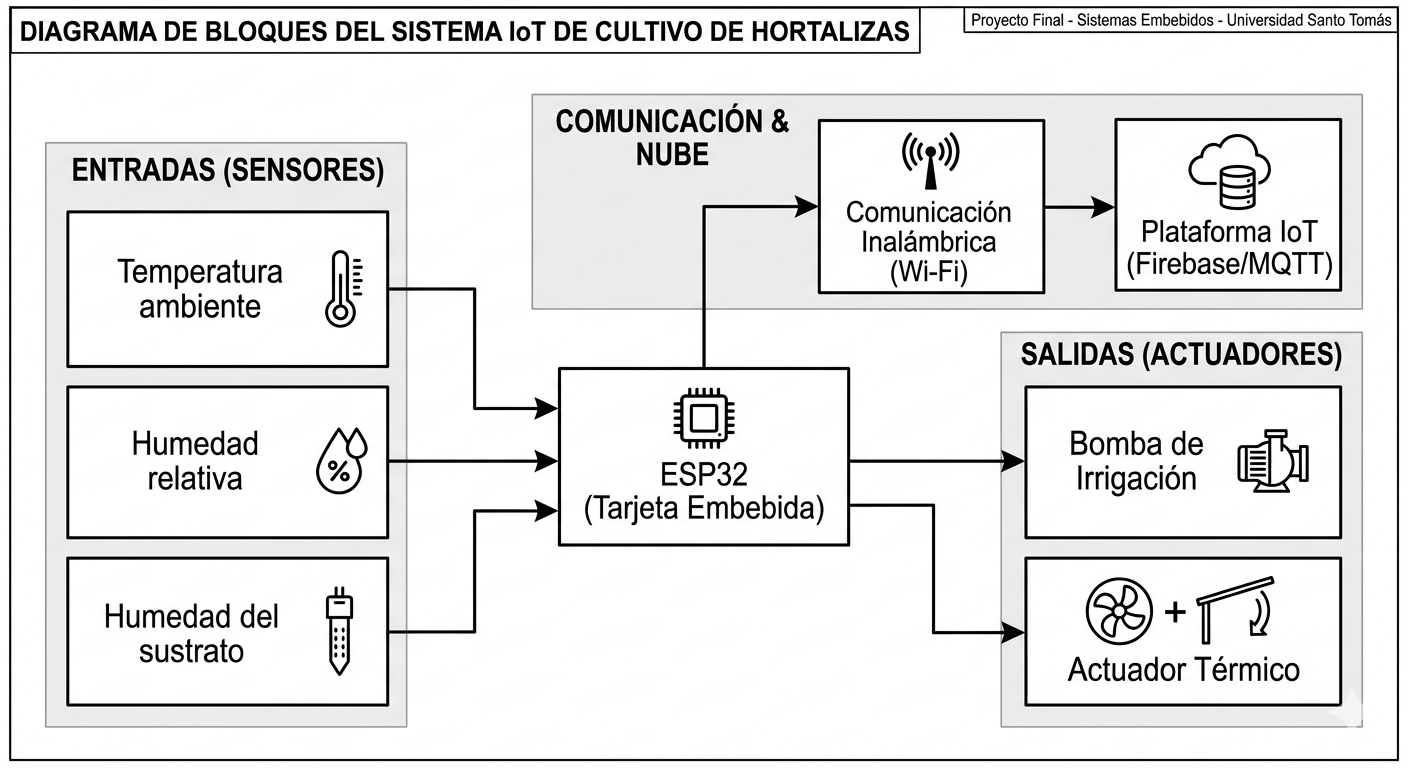
\includegraphics[width=0.85\columnwidth]{Diagrama_General.png}
    \caption{Diagrama general del sistema.}
    \label{fig:diagrama_general}
\end{figure}

% --- 1.5  Selección de Hardware y CAD -------------------------
\subsubsection{Selección de Hardware y Diseño CAD}

\noindent
\textbf{Tarjeta: ESP32.} Elegida por su conectividad Wi-Fi
integrada y sus múltiples canales ADC. La
figura~\ref{fig:IMAGEN_CAD} muestra el diseño CAD del sistema
estructural básico.

\begin{figure}[H]
    \centering
    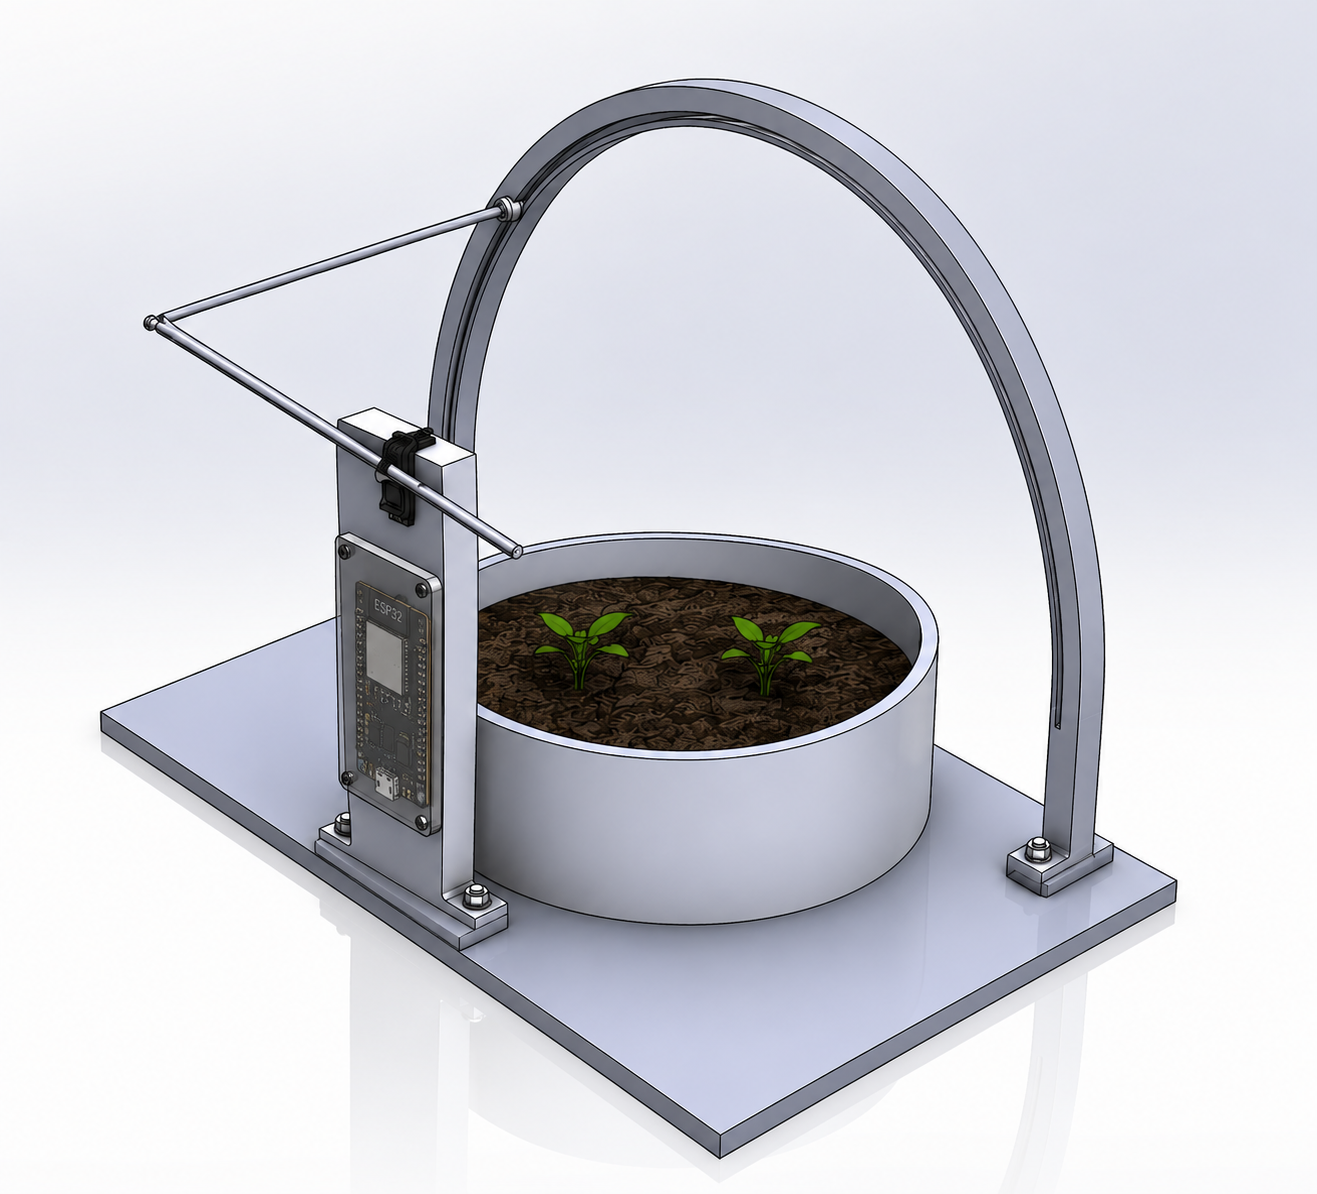
\includegraphics[width=0.85\columnwidth]{images/IMAGEN_CAD.png}
    \caption{CAD del sistema básico estructural.}
    \label{fig:IMAGEN_CAD}
\end{figure}

% --- 1.6  Lógica de Control -----------------------------------
\subsubsection{Lógica de Control}

\noindent
El diagrama de flujo de la figura~\ref{fig:diagrama_flujo}
describe el comportamiento del firmware embebido.

\begin{figure}[H]
    \centering
    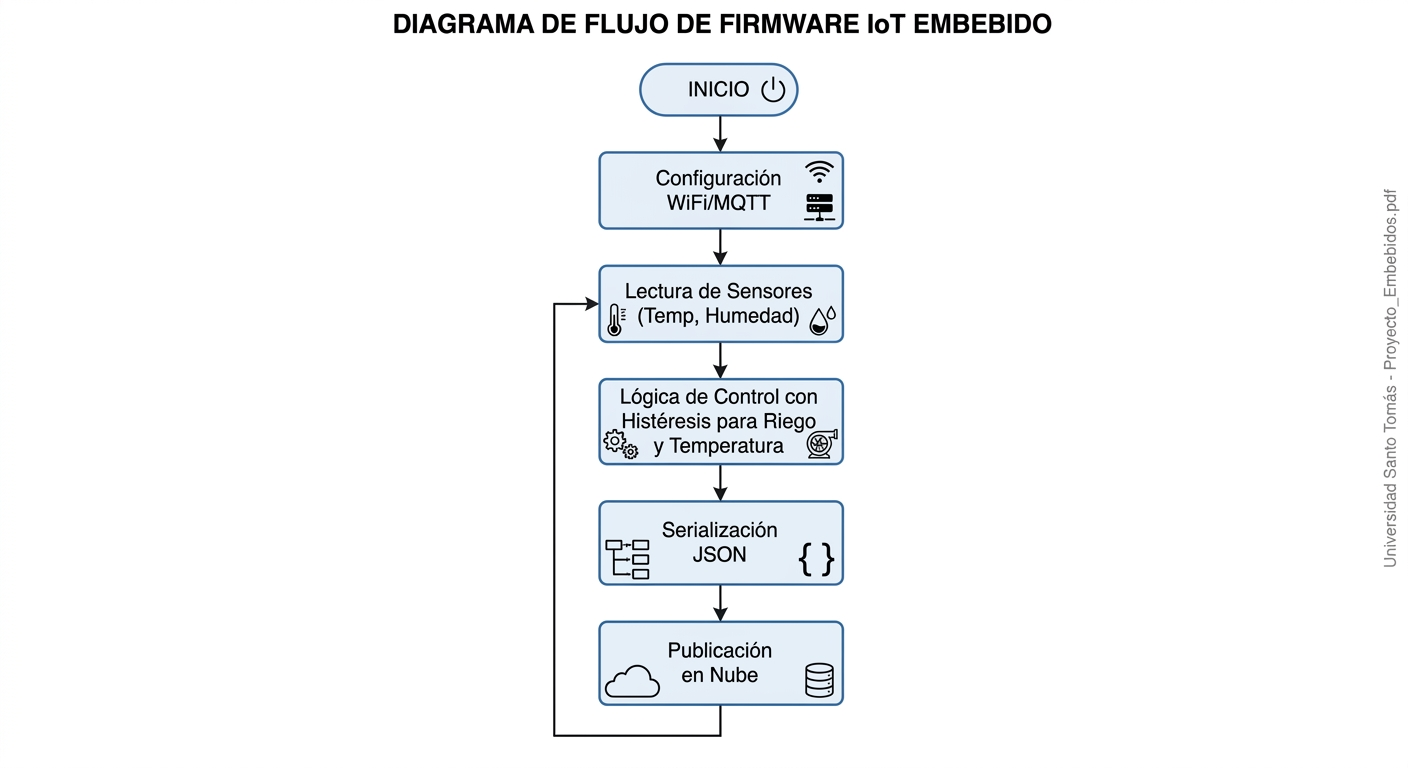
\includegraphics[width=0.85\columnwidth]{Diagrama_flujo.png}
    \caption{Diagrama de flujo del firmware.}
    \label{fig:diagrama_flujo}
\end{figure}

% =============================================================
\subsection{Entregable 2}
% =============================================================


\subsubsection{Codigo Fuente}
% TODO: Completar contenido del Entregable 2.
% Fin del bloque LaTeX para pegar


\section{Resultados}\label{sec:resultados}
  \input{section/results}

\section{Conclusiones}\label{sec:conclusiones}
  \input{section/conclusions}

% La sección de agradecimientos es opcional y no está numerada.
\section*{Agradecimientos}\label{sec:agradecimientos}
  \input{section/acknoledgment}

% ===================================================================
% BIBLIOGRAFÍA
% ===================================================================
% Define el estilo de la bibliografía (IEEEtran es el estándar).
% Añade tus referencias en el archivo 'reference.bib'.
\bibliographystyle{IEEEtran}


\footnotesize\bibliography{reference.bib}
\section{Anexos}\label{sec:anexos}
  \subsection{Código Reto 1}
\label{anexo:codigo1}
\lstinputlisting[
language=C,
breaklines=true,
basicstyle=\ttfamily\tiny,
inputencoding=utf8,
extendedchars=true
]{section/Anexos/Reto1.ino}

\subsection{Código Reto 2}
\label{anexo:codigo2}
\lstinputlisting[
language=C,
breaklines=true,
basicstyle=\ttfamily\tiny,
inputencoding=utf8,
extendedchars=true
]{section/Anexos/Reto2.ino}

\subsection{Código Reto 3}
\label{anexo:codigo3}
\lstinputlisting[
language=C,
breaklines=true,
basicstyle=\ttfamily\tiny,
inputencoding=utf8,
extendedchars=true
]{section/Anexos/Reto3.ino}
\end{document}
